\section[Fundamental Concepts]{\hyperlink{toc}{Fundamental Concepts}}
\subsection{The Beginnings of Quantum Mechanics}
Before we dive headfirst into the formalism of quantum mechanics, let us first review the first steps of the field as taken in the early 1900s. 

Our first founder is Max Planck; the problem at hand was the problem of the blackbody radiation spectrum. The two pre-existing laws (derived from thermodynamics arguments alone) predicting the BBR intensity as a function of wavelength/frequency were flawed. The first was Wien's law (1896):
\begin{equation}
    I_{\text{Wien}}(\lambda, T) \sim \frac{1}{\lambda^5}\exp(-\frac{1}{\lambda T}) % I(\lambda, T) = \frac{2hc^2}{\lambda^5}e^{-\frac{hc}{\lambda k_B T}}
\end{equation}
which agreed with low wavelength/high frequency data well but failed to accurately describe high wavelength/low frequency emission. The second was Rayleigh-Jeans' law (1900):
\begin{equation}
    I_{\text{RJ}}(\lambda, T) \sim \frac{T}{\lambda^4} % I(\lambda, T) = \frac{2ck_B T}{\lambda^4}
\end{equation}
which agreed with high wavelength/low frequency data well but failed to accurately describe low wavelength/high frequency emission\footnote{It should be noted however that a full-derivation of the Rayleigh-Jeans law did not occur until 1905, at which point Planck had already established the more correct explanation.}. In fact, the intensity as predicted by Rayleigh-Jeans' diverges at low $\lambda$, leading to the (obviously) erroneous conclusion that the total energy emitted by a black body is infinite; the so-called ``ultraviolet catastrophe''.

In order to solve this problem, in 1900 Planck proposed a quantum hypothesis; that light carries energy in individual packets, or quanta. In particular, for light of frequency $f$, each quanta carries energy:
\begin{equation}
    E = hf.
\end{equation}
Combining this quantum hypothesis with the Boltzmann supression of high-energy states (from thermodynamics), Planck's law was then derived to be:
\begin{equation}
    I_{\text{Planck}}(\lambda, T) = \frac{2hc^2}{\lambda^5}\frac{1}{\exp(\frac{hc}{\lambda k_B T}) - 1}
\end{equation}
which agrees with the BBR spectrum data across all frequencies\footnote{Further, we can observe that Planck's law agrees with Wien's law in the high-frequency limit, and with Rayleigh-Jeans' law in the low-frequency limit.}. It should also be noted that the integral over all $f$ of the above radiance law yields is finite, resolving the ultraviolet catastrophe. 

\begin{figure}[htbp]
    \centering
    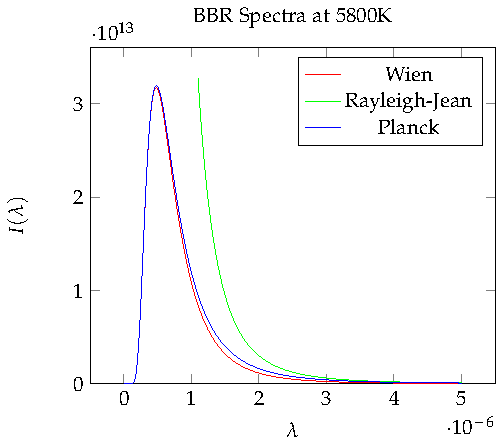
\includegraphics[]{Images/fig-BBRspectra.pdf}
    \caption{Plots of the black body emission spectra at $T = 5800\mathrm{K}$ (the approximate temperature of the surface of the sun) as predicted by Wien's Law, Rayleigh-Jean's Law, and Planck's Law. Planck's Law was found to agree with experimental observations for all wavelengths. Wien's Law agrees with observations well in the short wavelength limit but fails for long wavelengths. Rayleigh-Jean's Law agrees with observations in the long wavelength limit but fails at short wavelengths, and in fact the predicted emitted energy diverges.}
    \label{fig-BBRspectra}
\end{figure}


\noindent
In the above discussion, we have introduced Planck's constant. It has numerical value\footnote{which is the set/absolute (rather than measured) value of the Planck constant as per the 2018 redefinition of SI units.}:
\begin{equation}
    h = 6.626070040 \times 10^{-34}\si{J.s}
\end{equation}
$h$ is quantified as ``small''. What exactly does small mean in this context? For comparison, $1\si{eV}$ is the kinetic energy of an electron acquired in a voltage drop of a Volt, $0.035\si{eV}$ is the average kinetic energy of an atom at room temperature (from $E_k = \frac{3}{2}k_B T$) and $2.4\si{eV}$ is the energy of a single photon from the middle of the visible spectrum ($600 \si{THz}$). The energy of a single photon, which depends on $h$, is in other words ``typical'' of microscopic phenomena.

Planck's quantum hypothesis would be confirmed in Einstein's (Nobel-prize winning) 1905 explanation of the photoelectric effect (which you likely covered in detail in a previous course in modern physics); namely that quanta of light transfer energy $E = hf$ to electrons in the metal, kicking them out\footnote{Provided of course that $hf > \Phi$ where $\Phi$ is the ``work function'' of the metal.}.

Our second founder of interest is DeBroglie. In 1924, he postulated that matter could behave like a wave, positing the DeBroglie wavelength relation:
\begin{equation}
    p = \frac{h}{\lambda}.
\end{equation}
The so-called ``wave-particle'' duality would be confirmed in 1927 by the Davisson-Germer experiment, which saw peaks of electron intensity at distinct angles, showing that electrons scatter in the same nature as photons.

Our third founder of interest is Schr\"{o}dinger, who postulated the Schr\"{o}dinger equation (expressed below in the position basis) in 1926:
\begin{equation}
    i\hbar \dpd{}{t}\psi(\v{r}, t) = \left[\frac{-\hbar^2}{2m}\nabla^2 + V(\v{r}, t)\right] \psi(\v{r}, t).
\end{equation}
It should be noted that this is one of the two core formulas of non-relativistic quantum mechanics, and is the quantum-mechanical equivalent of Newton's laws. It however does not cover the effects of special relativity (for which we defer the reader to a future course on quantum field theory) or quantum measurement (which we shall address now). 

An illuminating demonstration of quantum measurement takes the form of the Stern-Gerlach experiment (first carried out in 1921/1922; see \href{https://physicstoday.scitation.org/doi/10.1063/1.1650229}{this article} for more historical background). In this experiment, silver atoms are heated and escape from an oven with uniform velocity. The beam of atoms then pass through an inhomogenous magnetic field (generated by an asymmetric pair of magnetic pole pieces) where they are deflected, before hitting a screen where their position is recorded. 

\begin{figure}[htbp]
    \centering
    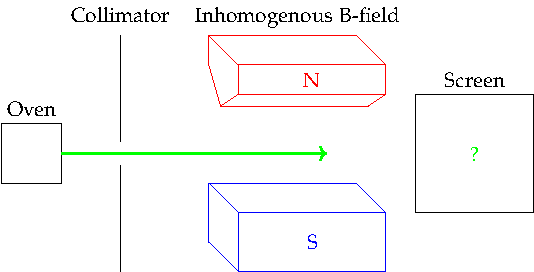
\includegraphics[]{Images/fig-SGexpsketch.pdf}
    \caption{Illustration of the Stern-Gerlach experiment. Silver (Ag) atoms are heated in an oven and escape, and pass through a collimator to form a narrow beam. They then pass through an inhomogenous magnetic field which deflects the atoms. The position of the atoms is then recorded when they hit the screen.}
    \label{fig-SGexpsketch}
\end{figure}

Why are silver atoms used for this experiment? Moreover, what exactly is being measured? For this, we consider a simplified model of the atom (which will suffice for the purposes of explaining this experiment). Silver atoms consist of 47 electrons in the shell, and 47 protons and 61 neutrons in the nucleus. A first guess of the mechanism of the atoms being deflected by the magnetic field may be a Lorentz force effect; however this is not the case as the atoms are electrically neutral. Instead, the silver atom has a single unpaired electron which has an intrinsic angular momentum, known as spin. In particular, the electron is spin-1/2\footnote{We will return to a more detailed discussion of angular momentum and spin at a later portion of the course}. This provides the silver atom with a net magnetic moment $\gv{\mu}$ proportional to the electron spin\footnote{The astute reader may question why the spin of the unpaired proton in the nucleus has no contribution to the net magnetic moment. This is due to the fact that the proportionality factor between the spin and magnetic moment has a factor of inverse mass. Since the proton is 1836 times heavier than the electron, the proton's magnetic moment contribution is negligeble compared to the electron's.} $\v{S}$:

\begin{equation}
    \gv{\mu} \propto \v{S}.
\end{equation}
We then recall from electromagnetism that a magnetic dipole $\gv{\mu}$ in a magnetic field $\v{B}$ has interaction energy:
\begin{equation}
    E = -\gv{\mu} \cdot \v{B}.
\end{equation}
We can then find the force that the dipole feels by taking the (negative) gradient of the energy:
\begin{equation}
    \v{F} = -\gv{\nabla}(-\gv{\mu} \cdot \v{B}) = \mat{\dpd{}{x}(\gv{\mu} \cdot \v{B}) \\ \dpd{}{y}(\gv{\mu} \cdot \v{B}) \\ \dpd{}{z}(\gv{\mu} \cdot \v{B})}.
\end{equation}
Ignoring the magnetic fields that are not in the $z$-direction, we find the force on the silver atoms in the $z$-direction to be:
\begin{equation}
    F_z = \mu_z \dpd{B_z}{z}.
\end{equation}
So in the inhomogenous field produced by the asymmetric magnets, the silver atoms should feel an up/downwards force depending on the direction of $\v{S}$ (which determines $\mu_z$). 

\begin{figure}[htbp]
    \centering
    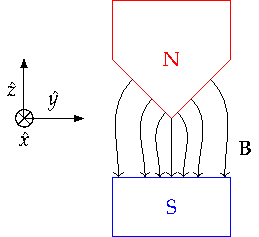
\includegraphics[]{Images/fig-SGexpmagnet.pdf}
    \caption{The inhomogenous magnetic field used in the Stern-Gerlach experiment, which deflects the silver atoms due to their magnetic dipole moment proportional to electron spin.}
    \label{fig-SGexpmagnet}
\end{figure}

Classically, the magnetic moment $\v{\mu}$ can point in any direction, and therefore $\mu_z$ ranges continuously from $+\abs{\gv{\mu}}$ to $-\abs{\gv{\mu}}$. Hence, the signature we would expect on the Stern-Gerlach experiment screen (wherein the vertical position of the atoms on the screen corresponds to a measurement of the $z$-component of the magnetic moment) would be a continuous band, as seen in the left of Fig. 1.4 below. However, this is \emph{not} what is observed; instead the experimental result was two discrete dots with nothing in between, as seen in the right of the figure. 

\begin{figure}[htbp]
    \centering
    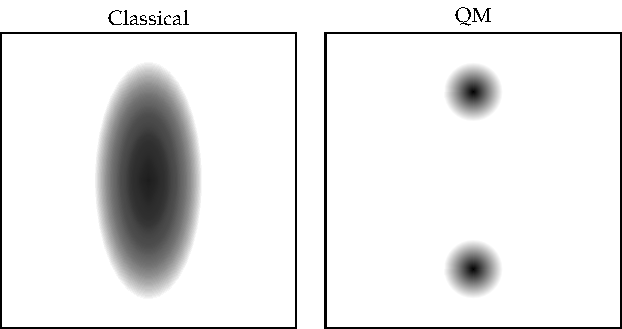
\includegraphics[]{Images/fig-SGexppredictions.pdf}
    \caption{Classical prediction (left) and quantum mechanical prediction (right) for the Stern-Gerlach experiment. The screen on the right was observed in experiment.}
    \label{fig-SGexppredictions}
\end{figure}

How do we interpret this result? We can associate the top dot with spins fully polarized upwards ($\uparrow$) and the bottom dot with spins fully polarized downwards ($\downarrow$). But why is there no signature for sideways pointing spins? We first will answer how a general spin (1/2) state can be represented. If $\ket{\uparrow}$ represents the spin-up state and $\ket{\downarrow}$ represents the spin-down state, then a general spin (and hence sideways spins) can be represented as complex superpositions of these two states, i.e.
\begin{equation}
    \ket{\psi} = \alpha\ket{\uparrow} + \beta\ket{\downarrow}
\end{equation}
where $\alpha, \beta \in  \CC$. What happens in a measurement is then that one element of this general superposition is picked with some probability; indeed, quantum measurement is a probabilistic process. Specifically, we find according to the Born rule that the probability that we measure the spin to be up is $p(\uparrow) = \abs{\uparrow}^2$ and the probability that we measure the spin to be down is $p(\downarrow) = \abs{\downarrow}^2$. Since we require that we measure either spin-up or spin-down, we obtain the normalization condition:
\begin{equation}
    p(\uparrow) + p(\downarrow) = \abs{\alpha}^2 + \abs{\beta}^2 = 1.
\end{equation}
The spin state after the measurement is then $\ket{\uparrow}$ or $\ket{\downarrow}$ respectively, according to the Dirac projection postulate. We will return to these two postulates of quantum mechanics and discuss them in full generality shortly. 

However, we will however make a second comment about measurement before concluding this section. Namely, we consider the case where we perform a repeated measurement of the $z$-component of the spin. As discussed above, the initial general spin state is given by $\ket{\psi} = \alpha\ket{\uparrow} + \beta\ket{\downarrow}$. We then measure the $z$-component of spin and the post-measurement spin state is $\ket{\uparrow}$ or $\ket{\downarrow}$ with probability $\abs{\alpha}^2$ and $\abs{\beta}^2$ respectively. What happens if we measure the $z$-component of spin again? We might think that again, we have probability $\abs{\alpha}^2$ of measuring spin-up and probability $\abs{\beta}^2$ of measuring spin-down. But this is \emph{not} the case. If we measured spin-up in the first measurement, we will measure spin-up in the second measurement with probability one. Similarly, if we measured spin-down in the first measurement, we will measure spin-down in the second measurement with probability one. Evidently, the first measurement has done something to the spin such that the measurement probabilities for the second measurement have been affected (they are not the same as the first). This tells us that quantum measurement is a active process that influences the state of the system we measure. Specifically, it is an irreversible process; there is no notion of ``undo''-ing the measurement to recover the initial (pre-measurement) state.


\subsection{Kets, Bras, and Hilbert Space}
Our goal of the initial stages of this course will be to understand the following table:

\begin{table}[htbp]
    \centering\begin{tabular}{|c|c|}
        \hline Quantum states & $\ket{\psi} \in \H$ 
        \\ \hline Evolution & $i\hbar\pd{}{t}\ket{\psi} = H\ket{\psi}$
        \\ \hline Measurement & $\ket{\psi} \mapsto \frac{\Pi_j \ket{\psi}}{\sqrt{\bra{\psi}\Pi_j\ket{\psi}}} \quad p(j) = \bra{\psi}\Pi_j\ket{\psi}$
        \\ \hline
    \end{tabular}
    \caption{Axioms of quantum mechanics, concerning states, evolution, and measurement.}
    \label{table-QMaxioms}
\end{table}

We will discuss the axioms for quantum states and quantum measurement in this chapter, and the axiom for quantum evolution (which readers may recognize as the Schr\"{o}dinger equation in basis independent form) in the next. It is worth noting that these are the \emph{fundamental postulates} of quantum mechanics; like Newton's laws of motion in classical mechanics, they cannot be derived. We are only able to interpret them, check if they are consistent, and work out the implications.

Let's start the axiom for quantum states; after all it will helpful to know what the objects of our interest are, before we start to work with them! 

\begin{axiombox}{: Quantum states}\label{axiom-states}
    Quantum states $\ket{\psi}$ are vectors (also called ``kets'') in a complex Hilbert space $\H$.
\end{axiombox}

The above axiom is only meaningful if we know what a Hilbert space is; its definition is below:

\begin{defbox}{: (Complex) Hilbert spaces}\label{def-Hilbertspaces}
    $\H$ is a (complex) Hilbert space if:
    \begin{enumerate}[(i)]
        \item $\H$ is a vector space over $\CC$
        \item $\H$ has an inner product
        \item $\H$ is complete (with respect to the metric induced by the norm induced by the inner product)\footnotemark - For the purposes of this course, this last point can be ignored.
    \end{enumerate}
\end{defbox}
\footnotetext{This is a technical qualification for the mathematicians in the crowd. An intuitive explanation for the curious; the inner product on a Hilbert spaces creates a notion of distance on the space. There are sequences (of vectors) that get closer together over time; completeness tells us that any such sequences (known as Cauchy sequences) must converge to a limit.}

Note that the vector space axioms for closure imply that $\forall \ket{\psi}, \ket{\phi} \in \H$ (where $\forall$ means ``for all'') and $\forall c \in \CC$, then $\ket{\psi} + \ket{\phi} \in \H$ and $c\ket{\psi} \in \H$. This tells us that the superposition of quantum states is well defined!

An example which we will return to time and time again (and have already encountered once) is the Hilbert space for a spin-1/2 system. In this case, $\H = \CC^2$. A question that may be brooding in the reader's mind may be ``why do we have to use complex numbers?''; one may indeed wonder if real Hilbert spaces may suffice to do quantum mechanics. The response is negative; we indeed need complex numbers! As an illustrative example, consider again the general spin-1/2 state $\ket{\psi} = \alpha\ket{\uparrow} + \beta\ket{\downarrow}$. Suppose we want a state that has equal probability to be measured spin-up or spin-down under a measurement of the $z$-component of spin. Since $p(\uparrow) = \abs{\alpha}^2$ and $p(\downarrow) = \abs{\beta}^2$, in order to have equal probability we must have $\abs{\alpha} = 1/\sqrt{2}$ and $\abs{\beta} = 1/\sqrt{2}$. A spin pointing in the $+x$ or $-x$ directions indeed has equal weight of up and down. Up to an overall (irrelevant) minus sign, without using complex numbers there are two ways to superimpose $\ket{\uparrow}$ and $\ket{\downarrow}$, from which we can define states corresponding to spins fully polarized in $\pm x$:

\begin{equation}\label{eq-xpm}
    \ket{x, \pm} = \frac{\ket{\uparrow} \pm \ket{\downarrow}}{\sqrt{2}}.
\end{equation}
However, the $\pm \hat{x}$ and $\pm \hat{y}$ vectors lie in the same $z = 0$ plane, and by symmetry we should require that the $\ket{y, \pm}$ would also have equal weights of $\ket{\uparrow}$ and $\ket{\downarrow}$. But if we limit ourselves to real numbers only, we have already exhausted all possible equal-weight combinations of $\ket{\uparrow}$ and $\ket{\downarrow}$ in Eq. \eqref{eq-xpm}. We therefore require complex  numbers to represent all possible states (and indeed, we find that $\ket{y, \pm} = \frac{\ket{\uparrow} \pm i \ket{\downarrow}}{2}$).

Having motivated the ``complex'' in the complex vector space part of the definition of Hilbert spaces, let us now motivate the inner product. We want some way to compare quantum states to one another. Our geometric intuition tells us that the states $\ket{\uparrow}$ and $\ket{\nearrow}$ are ``close'' to each other, while $\ket{\uparrow}$ and $\ket{\downarrow}$ are very ``different''. In order to make this intuition rigorous, we define the inner product, and as a prerequisite we define the dual correspondence.

\begin{defbox}{: Dual correspondence}\label{def-dualcorrespondence}
    To each vector space $\H$, there exists a dual vector space $\H^*$. There is a one-to-one correspondence\footnotemark between the kets $\ket{\psi} \in \H$ and the bras\footnotemark $\bra{\psi} \in \H^*$. We call this the \emph{dual correspondence}, and write it as follows:
    \begin{equation}
        \ket{\psi} \DC \bra{\psi}.
    \end{equation}
    It has the following properties:
    \begin{enumerate}[(i)]
        \item $\ket{\psi} + \ket{\phi} \DC \bra{\psi} + \bra{\phi}$
        \item $c\ket{\psi} \DC c^*\bra{\psi}$
    \end{enumerate}
    where the $*$ denotes complex conjugation.
\end{defbox}
\footnotetext{Formally, this follows from the Riesz Representation Theorem. But for the purposes of this course, we take this one-to-one correspondence as a postulate. Curious readers can find discussions/proofs of the theorem in any text on functional analysis, or mathematical quantum theory.}
\footnotetext{Given such names because $\braket{}{}$ is a bracket - bra-ket. Physicists remain unmatched in their sense of humour.}

Having established the dual correspondence, we may now define the inner product:

\begin{defbox}{: Inner product}\label{def-innerproduct}
    We define the inner product between $\ket{\psi} \in \H$ and $\ket{\phi} \in \H$ as:
    \begin{equation}
        \braket{\phi}{\psi} \in \CC
    \end{equation}
    with the properties:
    \begin{enumerate}[(i)]
        \item $\braket{\phi}{\psi} = \braket{\psi}{\phi}^*$
        \item $\braket{\psi}{\psi} \geq 0, \forall \ket{\psi} \in \H$
        \item $\braket{\psi}{\psi} = 0 \implies \ket{\psi} = \v{0}$.
    \end{enumerate}
\end{defbox}
Note that $\v{0}$ in the above definition is the null ket (also known as the zero vector, which must be an element of the Hilbert space), where $\v{0} = 0\ket{\psi}, \forall \ket{\psi}$. It is an unphysical state. We normally work with normalized states, i.e. states $\ket{\psi}$ that satisfy $\braket{\psi}{\psi} = 1$. The null ket has inner product zero and cannot be normalized.

As a first use of the inner product, let us return to our initial motivation for obtaining the ``likeness'' of states. For normalized states, it follows (and we will later prove) that:
\begin{equation}
    0 \leq \abs{\braket{\phi}{\psi}} \leq 1.
\end{equation}
We therefore can use the inner product as a method to evaluate the likeness of states. $\braket{\phi}{\psi} = 0$ means that $\ket{\psi}$ and $\ket{\phi}$ are maximally different, and $\abs{\braket{\phi}{\psi}} = 1$ corresponds to $\ket{\psi}$ and $\ket{\phi}$ being the same.

Next, we move onto a discussion of bases of Hilbert spaces. Since Hilbert spaces are vector spaces, they admit a basis. Let us recall what a basis is.

\begin{defbox}{: Basis}\label{def-basis}
    A \emph{basis} $\mathcal{B}$ of $\H$ is a set of states $\mathcal{B} = \set{\ket{b_j}}_j$ such that every state $\ket{\psi} \in \H$ can be written in the form:
    \begin{equation}\label{eq-expandpsibasis}
        \ket{\psi} = \sum_j \psi_j \ket{b_j}
    \end{equation}
    with $\psi_j \in \CC \forall j$, and the expansion on the RHS is unique.

    $\abs{\mathcal{B}}$ is the dimension of $\mathcal{H}$\footnotemark. 
\end{defbox}
\footnotetext{In the case where the Hilbert space is infinite-dimensional, there are additional complications (and in fact, two different kinds of bases!) In general the work we do in this course works perfectly well in the finite-dimensional case, and in the infinite dimensional case we will have to wave our hands a bit in order to avoid getting into the weeds of functional analysis; this is a physics course after all.}

Of particular interest to us will be orthonormal bases, or ONBs.

\begin{defbox}{: Orthonormal bases}\label{def-ONB}
    A basis $\mathcal{B} = \set{\ket{b_j}}_j$ is \emph{orthonormal} if
    \begin{equation}
        \braket{b_i}{b_j} = \delta_{ij}.
    \end{equation}
    where $\delta_{ij}$ is the Kronecker delta, defined as:
    \begin{equation}
        \delta_{ij} = \begin{cases}
            1 & i = j
            \\ 0 & i \neq j
        \end{cases}.
    \end{equation}

    One can obtain the expansion coefficients $\psi_j$ with respect to ONBs. Writing $\ket{\psi} = \sum_j \psi_j \ket{b_j}$ as in Eq. \eqref{eq-expandpsibasis} and taking the inner product of $\ket{\psi}$ with a vector $\ket{b_i}$ from the ONB, we have:
    \begin{equation}
        \braket{b_i}{\psi} = \sum_j \psi_j \braket{b_i}{b_j} = \sum_j \psi_j \delta_{ij} = \psi_i.
    \end{equation}
\end{defbox}

We will now prove a useful trick involving ONBs.

\begin{propbox}{: Resolution of the identity}\label{thm-residentity}
    For all ONBs $\set{\ket{b_j}}_j$, the following relation holds:
    \begin{equation}
        \sum_j \dyad{b_j}{b_j} = \II
    \end{equation}
    where $\II$ is the identity operator on the Hilbert space.
\end{propbox}

\begin{proof}
    Recall that $\ket{\psi} = \sum_j \psi_j \ket{b_j}$ for any $\ket{\psi} \in \H$ and for any basis $\set{\ket{b_j}}_j$ of $\H$. Further, recall that $\psi_j = \braket{b_j}{\psi}$ if the basis is orthonormal. Hence we have that:
    \begin{equation}
        \ket{\psi} = \sum_j \braket{b_j}{\psi}\ket{b_j} = \sum_j \ket{b_j}\left(\braket{b_j}{\psi}\right) = \sum_j \left(\dyad{b_j}{b_j}\right)\ket{\psi} = \left(\sum_j \dyad{b_j}{b_j}\right)\ket{\psi}.
    \end{equation}
    Since the above relation holds for all $\ket{\psi}$, it follows then that $\sum_j\dyad{b_j}{b_j}$ is the identity as claimed.
\end{proof}

At this point in the course, the reader may be wondering what happened to quantum \emph{wavefunctions}\footnote{Though this nomenclature of ``wavefunction'' is arguably a misnomer; the Schr\"{o}dinger equation does not contain second order derivatives in time, as a wave equation would.}; the central objects of interest have instead been quantum states, without a wavefunction in sight. We now elucidate the connection between the two.

\begin{defbox}{: Wavefunctions}
    Consider (as before) expanding $\ket{\psi}$ in a ONB $\set{\ket{b_j}}_j$. We then have:
    \begin{equation}
        \ket{\psi} = \sum_j \ket{b_j}\braket{b_j}{\psi}.
    \end{equation}
    Therein, $\psi_j = \psi(j) = \braket{b_j}{\psi}$ is the \emph{wavefunction}; a wavefunction is just a quantum state expanded in a given ONB. 
\end{defbox}

A particularly important (and familiar) example is using the position basis. Consider the resolution of the identity involving position:
\begin{equation}
    \int \mathrm d x \dyad{x}{x} = \II.
\end{equation}
For any $\ket{\psi}$, we then have:
\begin{equation}
    \ket{\psi} = \int \mathrm d x \ket{x}\braket{x}{\psi}.
\end{equation}
Where $\braket{x}{\psi} = \psi(x)$ is the position wavefunction, which played a central role in your first course in quantum mechanics. However, the reader should now recognize that $\ket{\psi}$ is a more fundamental object than this wavefunction, as it not only contains the information for $\psi(x)$ but also for $\tilde{\psi}(p)$ (the momentum wavefunction) or any other wavefunction; any wavefunction is just the expansion coefficients of the state in a given basis.

We have now established quite a bit of machinery to discuss quantum states, but have not done anything with the states; let's change that by discussing measurements! In a quantum measurement, the alternatives $\set{\ket{m_j}, j \in \text{ Outcomes }}$ for the states after measurement will:
\begin{itemize}
    \item Form a basis
    \item And are pairwise orthogonal, i.e. $\braket{m_i}{m_j} = 0, \forall i \neq j$. 
\end{itemize}
With the necessary mathematical formalism under our belt, we can now state a first version of the Dirac postulate and Born rule axioms.

\begin{axiombox}{: Quantum measurement (version 1)}\label{axiom-measurementver1}
    \textbf{Dirac postulate:} Under quantum measurement, the measured quantum state $\ket{\psi}$ is probabilistically changed into one of a number of alternatives $\set{\ket{m_j}}_j$, with:
    \begin{equation}
        \braket{m_i}{m_j} = \delta_{ij}.
    \end{equation}
    Note that $\set{\ket{m_j}}_j$ forms an ONB.
    
    \textbf{Born rule:} Given a quantum state $\ket{\psi}$, the probability for obtaining outcome $j$, corresponding to post-measurement state $\ket{m_j}$, is:
    \begin{equation}
        p_j = \abs{\braket{m_j}{\psi}}^2.
    \end{equation}
\end{axiombox}

There are now two questions that may arise. The first is that the statement of the Dirac projection postulate and the Born rule do not match that found in Table \ref{table-QMaxioms}. The second question concerns the post-measurement states $\set{\ket{m_j}}_j$; namely, how are they are determined? We will address the latter question first, and build up the formalism to state the measurement axioms in full generality. To this end, we move to a discussion of linear operators, which describe quantum mechanical observables and evolution. 

\subsection{Operators and Observables}

\begin{defbox}{: Linear operators}\label{def-linops}
    $A$ is an \emph{operator} that acts on a Hilbert space $\H$ if $\forall \ket{\psi} \in \H$, $A\ket{\psi} \in \H$. $A$ is $\emph{linear}$ if:
    \begin{equation}
        A(\alpha\ket{\psi} + \beta\ket{\phi}) = \alpha(A\ket{\psi}) + \beta(A\ket{\phi})
    \end{equation}
    $\forall \ket{\psi}, \ket{\phi} \in \H$ and $\forall \alpha, \beta \in \CC$.
\end{defbox}

A point of notation; we will use capital letters to denote operators in this course. Some sources also use hats to denote this (e.g. $\hat{A}$). Note that linear operators can be added and multiplied (more accurately, composed) to yield other linear operators. They are associative and distributive under these operations, i.e. for all linear operators $A, B, C$ we have:
\begin{equation}
    (A + B) + C = A + (B + C)
\end{equation}
\begin{equation}
    (AB)C = A(BC)
\end{equation}
\begin{equation}
    A(B + C) = AB + AC.
\end{equation}
However, note that in general operators are \emph{not} commutative, that is:
\begin{equation}
    AB \neq BA.
\end{equation}

Quantum mechanical observables are a specific type of linear operators; namely, they are Hermitian. In order to make sense of this, we introduce two more definitions.

\begin{defbox}{: Hermitian adjoint}\label{def-adjoint}
    The \emph{Hermitian adjoint} $A^\dagger$ of a linear operator $A$ is defined via the dual correspondence:
    \begin{equation}
        A\ket{\psi} \DC \bra{\psi}A^\dagger.
    \end{equation}
\end{defbox}

\begin{defbox}{: Hermitian operators and observables}\label{def-observables}
    An operator $A$ is \emph{Hermitian} if:
    \begin{equation}
        A^\dagger = A.
    \end{equation}
    Quantum mechanical \emph{observables} (such as position, momentum, spin, and energy) are Hermitian operators.
\end{defbox}

In general, acting on a state with an operator changes the state, and the new state is not necessarily proportional to the original state, i.e:
\begin{equation}
    A\ket{\psi} \not\propto \ket{\psi}.
\end{equation}
However, for special states known as eigenstates of an operator, this is indeed the case.

\begin{defbox}{: Eigenstates and eigenvalues}\label{def-eigstates}
    An \emph{eigenstate} $\ket{a}$ of a linear operator $A$ is a state that satisfies:
    \begin{equation}
        A\ket{a} = a\ket{a}.
    \end{equation}
    Therein, $a \in \CC$ is the \emph{eigenvalue} corresponding to that eigenstate. The null vector $\v{0}$ is excluded from being an eigenvector.
\end{defbox}

Having defined these objects, we state (but do not prove) an important theorem concerning observables:

\begin{thmbox}{: Diagonalization/Spectral theorem}
    A Hermitian operator $A$ (i.e. any observable) can be diagonalized; that is, it is able to be written as:
    \begin{equation}
        A = \sum_i a_i \dyad{a_i}{a_i}
    \end{equation}
    Where the eigenvectors $\set{\ket{a_i}}$ of $A$ forms an orthonormal basis\footnotemark (an \emph{eigenbasis}) and $a_i$ are the corresponding eigenvalues.
\end{thmbox}
\footnotetext{If the eigenvalues of $A$ are non-degenerate, then the set of eigenstates of $A$ are automatically mutually orthogonal, as we prove in the next theorem. If $A$ has degenerate eigenvalues, two eigenstates with the same eigenvalue are not necessarily guaranteed to be orthogonal, but we are still able to choose eigenstates (picking orthogonal vectors from the degenerate subspaces) to form an ONB out of the eigenstates; so we need not worry too much.}
With some more machinery developed, we can more carefully state the Dirac postulate and the Born rule.

\begin{axiombox}{: Quantum measurement (version 2)}
    \textbf{Dirac postulate:}
    \begin{enumerate}
        \item Each possible outcome of the measurement of an observable $A$ is an eigenvalue of $A$.
        \item If the eigenvalue $a$ is found in the measurement, then the post measurement state is an eigenvector $\ket{a}$ of $A$,
        \begin{equation}
            \ket{\psi} \mapsto \ket{a}
        \end{equation}
        satisfying
        \begin{equation}
            A\ket{a} = a\ket{a}.
        \end{equation}
    \end{enumerate}

    \textbf{Born rule:} Given an initial state of $\ket{\psi}$, the possibility for the measurement outcome $a_i$ occuring in a measurement of an observable $A$ (where $a_i$ is an eigenvalue of $A$) is:
    \begin{equation}
        p_i = \abs{\braket{a_i}{\psi}}^2.
    \end{equation}
\end{axiombox}

We reiterate that the eigenstate $\ket{a}$ is the possible post-measurement state, and the eigenvalue $a$ is the corresponding measurement outcome. As a concrete example, the spin-$z$ operator $S_z$ (for spin-1/2) systems has eigenstates $\ket{\uparrow}$ and $\ket{\downarrow}$, with corresponding eigenvalues of $+\hbar/2$ and $-\hbar/2$ (i.e. $S_z\ket{\uparrow} = +\hbar/2\ket{\uparrow}$, and likewise for $\ket{\downarrow}$). We may write $S_z$ in diagonal form as:
\begin{equation}
    S_z = \frac{\hbar}{2}(\dyad{\uparrow}{\uparrow} - \dyad{\downarrow}{\downarrow}).
\end{equation}
A measurement of the $z$ component of spin has two possible outcomes $\pm \hbar/2$, corresponding to post measurement states $\ket{\uparrow}/\ket{\downarrow}$. $\set{\ket{\uparrow}, \ket{\downarrow}}$ is an ONB, and we can expand a general state $\ket{\psi}$ in this basis as $\ket{\psi} = \alpha\ket{\uparrow} + \beta\ket{\downarrow}$. The Born rule then tells us that $p(\uparrow) = \abs{\braket{\uparrow}{\psi}}^2 = \abs{\alpha}^2$ and similarly that $p(\downarrow) = \abs{\beta}^2$. 

There are two points of consistency that the restatement of the Dirac postulate invites. First, an experiment should only have real-valued outcomes; an measurement shouldn't return a complex number. Second, it is not a priori immediate that the eigenstates/post-measurement states are mutually orthogonal, as the first statement of the postulate requires. Fortunately, there is a theorem that covers both.

\begin{thmbox}{}
    The eigenvalues of a Hermitian operator $A$ are real, and the eigenvectors of $A$ corresponding to distinct eigenvalues are orthogonal.
\end{thmbox}

\begin{proof}
    Consider two eigenstates $\ket{a}, \ket{a'}$ of $A$ (with corresponding eigenvalues $a, a'$). First, we make the observation that $\bra{a}A = \bra{a}a^*$. This follows as:
    \begin{equation}
        \bra{a}a^* \DC a\ket{a} = A\ket{a} = A^\dagger\ket{a} \DC \bra{a}A 
    \end{equation}
    where the first equality invokes that $\ket{a}$ is an eigenvector of $A$, and the second equality invokes the Hermicity of $A$. Since the dual correspondence is unique, we can compare the first and the last expressions to conclude that $\bra{a}A = \bra{a}a^*$. Next, we consider the number $\bra{a}A\ket{a'}$. We may write this as:
    \begin{equation}
        \bra{a}A\ket{a'} = \bra{a}(A\ket{a'}) = \bra{a}a'\ket{a} = a'\braket{a}{a'}
    \end{equation} 
    but by associativity, we can just as well write this as:
    \begin{equation}
        \bra{a}A\ket{a'} = (\bra{a}A)\ket{a'} = \bra{a}a^*\ket{a'} = a^*\bra{a}{a'}.
    \end{equation}
    Therefore we find that $a^*\bra{a}{a'} = a'\braket{a}{a'}$. From this we obtain that:
    \begin{equation}\label{eq-eigveccondition}
        (a^* - a')\braket{a}{a'} = 0.
    \end{equation}
    There are now two cases to consider.
    \begin{enumerate}[(I)]
        \item If $\ket{a} = \ket{a'}$, then $\braket{a}{a'} = \braket{a}{a} > 0$ (as $\ket{a}$ is an eigenvector, it cannot be a null vector). Therefore for Eq. \eqref{eq-eigveccondition} to be satisfied it must follow that $a^* = a$, i.e. $a$ is real.
        \item If instead $a \neq a'$, then $a^* \neq a'$ (as $a = a^*$), so for Eq. \eqref{eq-eigveccondition} to be satisfied it must follow that $\braket{a}{a'} = 0$. 
    \end{enumerate}
\end{proof}

We have now shown that the Dirac projection postulate is consistent with what we should expect out of measurements. However, we now clarify what is often a point of confusion, that being the difference between individual and averaged measurement outcomes. The dirac postulate states that given a state $\ket{\psi}$, a possible outcome of the measurement of an observable $A$ are eigenvalues $a$ of $A$. This speaks to possible outcomes in \emph{individual measurements}. The \emph{expectation value} is conceptualized quite differently.

\begin{defbox}{: Expectation values}
    The \emph{expectation value} $\avg{A}_\psi$ is the average outcome in the measurement of $A$ on $\ket{\psi}$, i.e.:
    \begin{equation}\label{eq-expectation}
        \avg{A}_\psi \coloneqq \sum_i p_i a_i
    \end{equation}
    where $p_i$ is the probability of measuring outcome $a_i$. We are able to write Eq. \eqref{eq-expectation} equivalently as:
    \begin{equation}\label{eq-expection2}
        \avg{A}_\psi = \sum_i \abs{\braket{a_i}{\psi}}^2 a_i = \sum_i \braket{a_i}{\psi}^* \braket{a_i}{\psi} a_i = \sum_i \braket{\psi}{a_i} a_i \braket{a_i}{\psi} = \bra{\psi}\left(\sum_i a_i \dyad{a_i}{a_i}\right)\ket{\psi} = \bra{\psi}A\ket{\psi}.
    \end{equation}
    where in the first equality we use the Born rule, and in the last equality we consider $A$ in diagonalized form.
\end{defbox}

The formalism of quantum mechanics is therefore well-suited to predict both individual and averaged measurement outcomes; but take care not to confuse them! In general $\avg{A}_\psi$ is \emph{not} a possible (individual) measurement outcome.

Up until now, we have considered both kets $\ket{\psi}$ and operators $A$ as abstract objects; however sometimes it is helpful to cast these into a more concrete form in order to do computations. We thus introduce the idea of matrix/vector representations.

Consider an ONB $\mathcal{B} = \set{\ket{b_i}}_i$, and consider an expression of the form $\ket{\phi} = A\ket{\psi}$. Inserting the resolution of the identity once on the left hand side and twice on the right hand side, we have:
\begin{equation}
    \left(\sum_i \dyad{b_i}{b_i}\right)\ket{\phi} = \left(\sum_i \dyad{b_i}{b_i}\right)A\left(\sum_j \dyad{b_i}{b_i}\right)\ket{\psi}
\end{equation}
Now redrawing some brakets we obtain:
\begin{equation}
    \sum_i \ket{b_i}(\braket{b_i}{\phi}) = \sum_{i}\sum_j \ket{b_i}(\bra{b_i}A\ket{b_j})(\braket{b_j}{\psi}).
\end{equation}
Now, we can consider $\braket{b_i}{\phi} = [\phi]_i$ and $\braket{b_j}{\psi} = [\psi]_i$ (where we use $[\cdot]$ to denote `representation of') as elements of column vectors $[\phi]$ and $[\psi]$, and $\bra{b_i}A\ket{b_j} = [A]_{ij}$ as elements of a matrix $[A]$. In other words, expanded out in the $\set{\ket{b_i}}_i$ basis, we can realize $[\phi]$ is the column vector obtained by multiplying the column vector $[\psi]$ by the matrix $[A]$.

Similarly, we can write for any bra $\bra{\tau}$ that:
\begin{equation}
    \bra{\tau} = \bra{\tau}\sum_i \dyad{b_i}{b_i} = \sum_i \braket{\tau}{b_i} \bra{b_i} = \sum_i [\tau]_i\bra{\tau}.
\end{equation}

This yields us the following way of thinking about bras/kets/operators:

\begin{table}[htbp]
    \centering\begin{tabular}{|c|c|}
        \hline Abstract Objects & Representation in ONB 
        \\ \hline Ket $\ket{\phi}$ & Column vector $[\phi]$
        \\ Operator $A$ & Matrix $[A]$
        \\ Bra $\bra{\tau}$ & Row vector $[\tau]$
        \\ \hline
    \end{tabular}
    \caption{Abstract objects and their representations when expanded out in a basis.}
    \label{table-ketsascolvecs}
\end{table}

However, do take note that a ket is \emph{not} equal to a column vector. The column vector is a representation of a ket, much in the same way that $\binom{1}{0}$ is not in itself a vector but instead a concrete (standard) representation of the abstract vector $e_1$. 

Let us supplement this discussion of matrix representations by returning to our favourite example of spin-1/2. Consider the ONB $\mathcal{B} = \set{\ket{\uparrow}, \ket{\downarrow}}$ of $\H = \mathbb{C}^2$. Making the identification that $\ket{\uparrow} \cong \binom{1}{0}$ and $\ket{\downarrow} \cong \binom{0}{1}$, for any $\ket{\psi} \H$ we then have that:
\begin{equation}
    \ket{\psi} \cong \mat{\braket{\uparrow}{\psi} \\ \braket{\downarrow}{\psi}} = [\psi]
\end{equation}
and for any linear operator $A$ acting on kets in $\H$ we have:
\begin{equation}
    A \cong \mat{\bra{\uparrow}A\ket{\uparrow} & \bra{\uparrow}A\ket{\downarrow} \\ \bra{\downarrow}A\ket{\uparrow} & \bra{\downarrow}A\ket{\downarrow}} = [A].
\end{equation}
Taking spin-$z$ operator $S_z$ as a concrete example, we can represent it in this basis as:
\begin{equation}
    S_z = \frac{\hbar}{2}\left(\dyad{\uparrow}{\uparrow} - \dyad{\downarrow}{\downarrow}\right) \cong \frac{\hbar}{2}\mat{1 & 0 \\ 0 & -1}.
\end{equation}
As another example, consider the spin-$x$ operator $S_x$. It has eigenstates:
\begin{equation}
    \ket{\pm} \coloneqq \frac{\ket{\uparrow} \pm \ket{\downarrow}}{\sqrt{2}}
\end{equation}
we can represent it as:
\begin{equation}
    S_x = \frac{\hbar}{2}\left(\dyad{+}{+} - \dyad{-}{-}\right) \cong \frac{\hbar}{2}\mat{0 & 1 \\ 1 & 0}.
\end{equation}

From the work we have done so far, it may have become clear that it is generally easiest to work in the eigenbasis of whatever observable is being considered. For example, if considering the measurement of the observable $S_z$, it is natural to work with the basis $\mathcal{B} = \set{\ket{\uparrow}, \ket{\downarrow}}$. This fact will continue to be true when we later consider Schr\"{o}dinger evolution of observables. However, there are times when there are multiple observables under consideration; in the measurement picture, this could be the sequential measurement of observable $O_1$ followed by the measurement of observable $O_2$\footnote{An similar setting of interest with Schr\"{o}dinger evolution could be the evolution of a quantum state under a Hamiltonian $H_1$ for some time $[t_0, t_1]$ followed by evolution by a different Hamiltonian $H_2$ for some time $[t_1, t_2]$.}. In this case, we have two different bases of interest, namely the eigenbasis of $O_1$ and the eigenbasis of $O_2$. We may then find it useful to consider a transformation between these bases; let us work through that now. 

Consider two ONBs defined by $\mathcal{B} = \set{\ket{b_i}}_i$ and $\mathcal{B}' = \set{\ket{a_j}}_j$, and some state $\ket{\psi} \in \mathcal{H}$. Inserting the resolution of identity $\II = \sum_j \dyad{a_j}{a_j}$ between the wavefunction $\braket{b_i}{\psi} = \psi_i$, we obtain:
\begin{equation}\label{eq-basistransform}
    \braket{b_i}{\psi} = \bra{b_i}\left(\sum_j \dyad{a_j}{a_j}\right)\ket{\psi} = \sum_j \braket{b_i}{a_j} \braket{a_j}{\psi}
\end{equation}
Now, $\braket{b_i}{\psi}$ can be viewed as elements of a column vector $[\psi]$ (whose components are the expansion coefficients of $\ket{\psi}$ in the basis $\mathcal{B}$), $\braket{a_i}{\psi}$ can be analogously viewed as the elements of a column vector $[\tilde{\psi}]$ (whose components are the expansion coefficients of $\ket{\psi}$ in the basis $\mathcal{B}'$), and $\braket{b_i}{a_j} = T_{ij}$ can be viewed as the matrix elements of a (matrix) representation of the transformation operator $T$ between the two bases. We can therefore write Eq. \eqref{eq-basistransform} as a matrix/vector equation:
\begin{equation}
    [\psi] = [T][\tilde{\psi}].
\end{equation}
The operator $T$ actually has a special property; namely, it is \emph{unitary}.

\begin{defbox}{: Unitary operators}
    A linear operator $U$ is \emph{unitary} if:
    \begin{equation}
        UU^\dagger = U^\dagger U = \II.
    \end{equation}
\end{defbox}
\begin{propbox}{}
    The basis transformation operator between bases $\mathcal{B} = \set{\ket{b_i}}_i$ and $\mathcal{B}' = \set{\ket{a_j}}_j$ defined as:
    \begin{equation}\label{eq-Tbasisagnostic}
        T = \sum_{n} \dyad{a_n}{b_n}
    \end{equation}
    which has matrix representation (in either $\mathcal{B}$ or $\mathcal{B}'$):
    \begin{equation}\label{eq-Tmatrix}
        [T]_{ij} = \braket{b_i}{a_j}
    \end{equation}
    is unitary.
\end{propbox}
\begin{proof}
    First, it should be clear from the basis agnostic definition in Eq. \eqref{eq-Tbasisagnostic} that $T$ is in fact a basis transformation operator, as by inspection it satisfies $T\ket{b_n} = \ket{a_n}$ for $n = 1, 2, \ldots d$. We next verify that it indeed has the claimed matrix representation; in the $\mathcal{B}$ basis, we have:
    \begin{equation}
        [T]_{ij} = \bra{b_i}T\ket{b_j} = \bra{b_i}\left(\sum_n \dyad{a_n}{b_n}\right)\ket{b_j} = \sum_n \braket{b_i}{a_n}\braket{b_n}{b_j} = \sum_n \braket{b_i}{a_n} \delta_{nj} = \braket{b_i}{a_j}
    \end{equation}
    and in the $\mathcal{B}'$ basis we have:
    \begin{equation}
        [T]_{ij} = \bra{a_i}T\ket{a_j} =  \bra{a_i}\left(\sum_n \dyad{a_n}{b_n}\right)\ket{a_j} = \sum_n \braket{a_i}{a_n}\braket{b_n}{a_j} = \sum_n \delta_{in}\braket{b_n}{a_j} = \braket{b_i}{a_j}
    \end{equation}
    so Eq. \eqref{eq-Tmatrix} indeed holds as claimed.
    
    We move onto the unitarity proof. We claim that the equality below:
    \begin{equation}\label{eq-adjointconjtranspose}
        [T^\dagger]_{kl} = [T]_{lk}^*
    \end{equation}
    holds \emph{in general} for any linear operator $T$. Note that Eq. \eqref{eq-adjointconjtranspose} reconciles the abstract notion of the Hermitian adjoint with the familiar operation of taking the conjugation transpose of a matrix (which you should have encountered in your linear algebra course). The equation follows from the definition of the Hermitian adjoint using the dual correspondence, and is left as an exercise for the reader. 

    Applying Eq. \eqref{eq-adjointconjtranspose} to the definition of $T$, we find:
    \begin{equation}\label{eq-Tdaggermatrixelements}
        [T^\dagger]_{kl} = [T]_{lk}^* = \braket{b_l}{a_k}^* = \braket{a_k}{b_l}.
    \end{equation}
    Next, we consider the matrix elements of the operator $T^\dagger T$:
    \begin{equation}
        [T^\dagger T]_{kj} = \sum_l [T^\dagger]_{kl}[T]_{lj} = \sum_l \braket{a_k}{b_l} \braket{b_l}{a_j} = \bra{a_k}\left(\sum_l \dyad{b_l}{b_l}\right)\ket{a_j}.
    \end{equation}
    where in the first equality we use the definition of matrix multiplication, and in the second equality we use Eq. \eqref{eq-Tdaggermatrixelements}. Recognizing the resolution of the identity, the above equation then becomes:
    \begin{equation}
        [T^\dagger T]_{kj} = \bra{a_k}\II\ket{a_j} = \braket{a_k}{a_j} = \delta_{kj}
    \end{equation}
    where in the last equality we use that $\set{\ket{a_j}}_j$ is an ONB. From $[T^\dagger T]_{kj} = \delta_{kj}$ we can conclude that  $T^\dagger T = \II$, and $TT^\dagger = \II$ can be shown analogously. We conclude that $T$ is unitary.
\end{proof}

Note that while this is our first encounter with unitarity, it will certainly not be our last; unitary operators will have a very large role to play when we consider Schr\"{o}dinger evolution.

As an example, let us solve for $T$ which transforms from the $S_z$ eigenbasis $\mathcal{B} = \set{\ket{\uparrow}, \ket{\downarrow}}$ to the $S_x$ eigenbasis $\mathcal{B} = \set{\ket{+} = \frac{\ket{\uparrow} + \ket{\downarrow}}{\sqrt{2}}, \ket{-} = \frac{\ket{\uparrow} - \ket{\downarrow}}{\sqrt{2}}}$. We may write it down in operator form as:
\begin{equation}
    T = \dyad{+}{\uparrow} + \dyad{-}{\downarrow}.
\end{equation}
To get a clearer picture, we can write down its matrix representation. Computing the inner products between the eigenvectors of $S_z$ and $S_x$, we obtain: 
\begin{equation}
    [T] = \mat{\braket{\uparrow}{+} & \braket{\uparrow}{-} \\ \braket{\downarrow}{+} & \braket{\downarrow}{-}} = \mat{\frac{1}{\sqrt{2}} & \frac{1}{\sqrt{2}} \\ \frac{1}{\sqrt{2}} & -\frac{1}{\sqrt{2}}} = \frac{1}{\sqrt{2}}\mat{1 & 1 \\ 1 & -1}.
\end{equation}
The above matrix representation is the same whether we choose the identification $\ket{\uparrow} \cong \binom{1}{0}, \ket{\downarrow} \cong \binom{0}{1}$ or $\ket{+} \cong \binom{1}{0}, \ket{-} \cong \binom{0}{1}$ (but note: this is NOT true of operators in general. For example the matrix representations of $S_z$ and $S_x$ will look different depending on the identifications chosen). It can be easily verified via matrix multiplication that $T$ is unitary, which is consistent with the general theorem we just proved. The $T$ above is a ubiquitous operator in the field of quantum computation, and is called the \emph{Hadamard operator}.

\subsection{Projectors and Measurement}
We now return to the setting of measurement to resolve an ambiguity that was left by version 2 of our measurement axioms. Namely, we ask ``what if the observable in question has degenerate eigenvalues?'' (Degenerate referring to the fact that two or more distinct eigenstates of an observable may have the same eigenvalues). To see why this is a problem with our current formulation, consider an operator $A$ with two distinct eigenstates $\ket{a}, \ket{\tilde{a}}$ such that:
\begin{equation}
    A\ket{a} = a\ket{a}, A\ket{\tilde{a}} = a\ket{\tilde{a}}.
\end{equation}
In our earlier formulation of the Dirac postulate, we claimed that a measurement of an observable $A$ with outcome/eigenvalue $a$ would change the quantum state to be an eigenstate with the corresponding eigenvalue. Now that there are two distinct eigenstates with the same eigenvalue, which eigenstate is chosen?

As a concrete example, we consider the $z$-component of spin for a spin-1 particle. The $S_z$ operator has three eigenstates, namely $\ket{+}, \ket{0}$ (this is \emph{not} the null ket/zero vector!) and $\ket{-}$ which forms a basis, and can be written as:
\begin{equation}
    S_z = \hbar(\dyad{+}{+} - \dyad{-}{-}).
\end{equation}
$\ket{+}$ has eigenvalue $+\hbar$, $\ket{0}$ has eigenvalue zero, and $\ket{-}$ has eigenvalue $-\hbar$. Now, consider the observable $S_z^2$. From $S_z$ above, we can deduce this to be:
\begin{equation}
    S_z^2 = \hbar^2(\dyad{+}{+} + \dyad{-}{-})
\end{equation}
Now, we find that both $\ket{+}$ and $\ket{-}$ have eigenvalue $+\hbar^2$. So, if we measured $S_z^2$ for a state $\ket{\psi}$ and got outcome $\hbar^2$, our current formulation is ill-equipped to deduce what the post-measurement state would be. In order to refine our formulation, we require the notion of a projector.

Another example (which we cannot discuss in full detail yet) is that of ``spooky action at a distance'' (coined by the one and only Einstein). In this setting, we have a two-particle system which is in an entangled Bell state (to be defined in full mathematical detail later; for now, take entangled to mean ``stronger than classically correlated'', or ''it is impossible to describe the individual subsystems/particles, and only the joint system can be described''). We then separate the two particles some great distance; say the Earth and moon. When we measure the particle on Earth (but do nothing to the particle on the moon), we find that upon knowing the Earth measurement outcome we \emph{immediately} know what the post-measurement state of the particle on the moon is. This seems counterintutive, and indeed, superliminal; it seems as though the measurement on Earth affects the state on the moon faster than the speed of light! While this setup does not actually turn out to violate special relativity (and indeed, we will prove later in the course that no quantum communication protocol can be superliminal), it is certainly of interest as depicting non-classical phenomenology. It turns out that the measurement of just the particle on Earth conducted in this setting corresponds to a measurement of a degenerate (joint) observable; we therefore also require a reformulation of our measurement axioms involving projectors here. Without further ado, let us define what a projector is.

\begin{figure}[htbp]
    \centering
    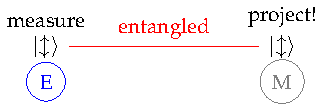
\includegraphics[]{Images/fig-spookyaction.pdf}
    \caption{Visualization of the ``spooky action at a distance'' scenario. A two-particle state is prepared in an entangled Bell state. The particles are then spatially separated a great distance; here depicted as one particle on the Earth and one particle in the moon. When the particle on Earth (and \emph{only} the particle on Earth) is measured, the entanglement structure of the state leads to the particle on the moon being projected into a post-measurement state that is immediately known to the experimenter on Earth based on their measurement outcome. The measurement conducted in this scenario of interest turns out to be one with degeneracy, and hence we require a reformulation of measurement in order to describe it.}
    \label{fig-spookyaction}
\end{figure}

\begin{defbox}{: Projectors}
    A linear operator $\Pi$ is a \emph{projector} if it satisfies:
    \begin{equation}\label{eq-projector}
        \Pi^2 = \Pi^\dagger = \Pi.
    \end{equation}
\end{defbox}
Below are examples of projectors in matrix representations:
\begin{equation}\label{eq-projectorexamples}
    \Pi_1 \cong \mat{1 & 0 & 0 \\ 0 & 0 & 0 \\ 0 & 0 & 0}, \quad \Pi_2 \cong \mat{1 & 0 & 0 \\ 0 & 1 & 0 \\ 0 & 0 & 0}.
\end{equation}
$\Pi_1$ is a rank 1 projector, while $\Pi_2$ is rank $2 > 1$. Why we call an operator with the properties in Eq. \eqref{eq-projector} a projector might not be obvious, but the nomenclature is elucidated by the above examples. A projector projects a state into a lower-dimensional subspace of the Hilbert space. $\Pi_1$ has the property of taking a three-dimensional vector and projecting it into a 1-dimensional subspace, while  $\Pi_2$ has the property of taking a three-dimensional vector and projecting it into a 2-dimensional subspace. $\mathbb{I}$ is a projector (though a trivial one), and is a projection from a space to itself. In Fig. \ref{fig-projectorvisualization} we visualize the action of $\Pi_1, \Pi_2$ for the case when our vector space is $\mathbb{R}^3$ (but one should keep in mind that this is for the sake of intuition, and the Hilbert spaces we use in quantum mechanics are, of course, complex).

\begin{figure}[htbp]
    \centering
    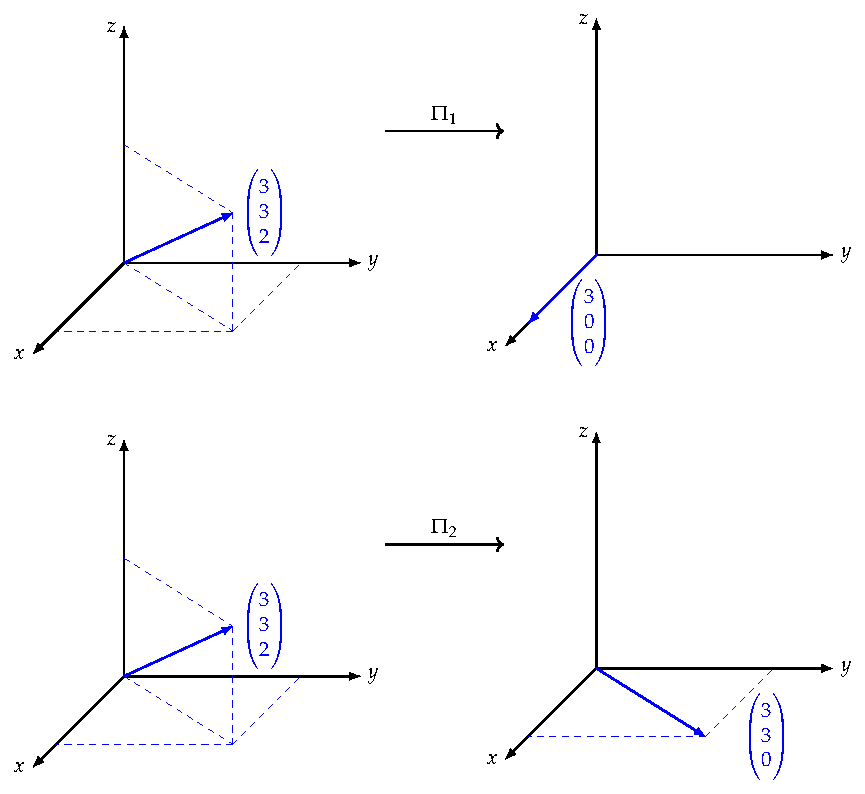
\includegraphics[]{Images/fig-projectorvisualization.pdf}
    \caption{Visualization of the action of projectors $\Pi_1, \Pi_2$ (as defined in Eq. \eqref{eq-projectorexamples}) on a vector in $\RR^3$. $\Pi_1$ can be visualized as projecting the given vector onto the one-dimensional subspace that is the $x$-axis subspace; preserving the $x$-component of the vector, and nullifying the $y$ and $z$-components. $\Pi_2$ can be visualized as projecting the given vector onto the two-dimensional subspace that is the $xy$-plane; preserving the $x$ and $y$ components of the vector and nullifying the $z$-component.}
    \label{fig-projectorvisualization}
\end{figure}

Now let's return to the bra-ket formalism and what projectors look like in this abstract setting. First, recall that we can write an observable $A$ in the form:
\begin{equation}
    A = \sum_i a_i \dyad{a_i}{a_i}
\end{equation}
where $\ket{a_i}$ is the eigenstate of $A$ corresponding to the eigenvalue $a_i$, and $\set{\ket{a_i}}_i$ is an ONB. In the non-degenerate case, each of the $a_i$s are distinct. However, in general degenerate eigenvalues (where $a_i = a_j$ for some $i, j$) are possible, and the current form of the expression does not make this particularly clear. With our knowledge of projectors, let us now rewrite the above as:
\begin{equation}
    A = \sum_a a \Pi_a
\end{equation}
where each of the $a$s are \emph{distinct} eigenvalues of $A$, and
\begin{equation}
    \Pi_a = \sum_{a_i = a} \dyad{a_i}{a_i}
\end{equation}
is the \emph{projector onto the eigenvalue-$a$ subspace}. Let us verify that these are indeed projectors. First, we verify that they are Hermitian:
\begin{equation}
    \Pi_a^\dagger = \left(\sum_{a_i = a} \dyad{a_i}{a_i}\right)^\dagger = \sum_{a_i = a} (\dyad{a_i}{a_i})^\dagger = \sum_{a_i = a} \dyad{a_i}{a_i} = \Pi_a.
\end{equation}
where in the second-to-last equality we use that $(\dyad{a}{b})^\dagger = \dyad{b}{a}$ (which follows immediately from the definition of the Hermitian adjoint; the proof is left to the reader!). Next, we show that they are idempotent (that is, they square to themselves):
\begin{equation}\label{eq-projectoridempotency}
    \Pi_a^2 = \left(\sum_{a_i = a} \dyad{a_i}{a_i}\right)^2 = \sum_{a_i = a} \sum_{a_j = a} \ket{a_i}\braket{a_i}{a_j}\bra{a_j} = \sum_{a_i = a}\sum_{a_j = a}\dyad{a_i}{a_j}\delta_{ij} = \sum_{a_i = a} \dyad{a_i}{a_i} = \Pi_a.
\end{equation}
So they are indeed projectors! In this form, we have decomposed the observable $A$ into the parts associated with each eigenvalue in a clear way. These projectors have some properties of note, described in the theorem below.

\begin{propbox}{}
    Let $\set{\Pi_a}_a$ be the set of projectors associated to an observable $A$ (with $\Pi_a = \sum_{a_i = a}\dyad{a_i}{a_i}$ being the projector onto the eigenvalue-$a$ subspace). These projectors are mutually orthogonal:
    \begin{equation}\label{eq-projectororthogonality}
        \Pi_i\Pi_j = \delta_{ij}\Pi_i
    \end{equation}
    and are complete:
    \begin{equation}
        \sum_a \Pi_a = \II.
    \end{equation}
\end{propbox}
\begin{proof}
    The idempotency of projectors covers the $i = j$ case in Eq. \eqref{eq-projectororthogonality}, and if $i \neq j$, then the expression is zero as eigenvectors of an observable $A$ corresponding to distinct eigenvalues are orthogonal. The completeness relation is merely a restatement of the resolution of the identity in terms of projectors.
\end{proof}

We are now ready to do our final, complete statement of the axioms of quantum measurement.

\begin{axiombox}{: Quantum measurement (version 3/final)}
    Let $A =  \sum_a a\Pi_a$ be the observable (a Hermitian operator) being measured,  where the $a$s are the eigenvalues of $A$ and $\set{\Pi_a = \sum_{a_i = a}\dyad{a_i}{a_i}}_a$ are the associated projectors onto the eigenvalue-$a$ subspaces. Let $\ket{\psi}$ be the pre-measurement state.

    \textbf{Dirac postulate:} If outcome $a$ is measured, then the post measurement state is given by:
    \begin{equation}\label{eq-diracpostulate}
        \ket{\psi} \mapsto \frac{1}{\sqrt{\bra{\psi}\Pi_a\ket{\psi}}}\Pi_a\ket{\psi}.
    \end{equation}

    \textbf{Born rule:} The probability of measuring outcome $a$ is given by:
    \begin{equation}\label{eq-bornrule}
        p(a) = \bra{\psi}\Pi_a\ket{\psi}.
    \end{equation}
\end{axiombox}
We have now reproduced the form of the Dirac postulate and Born rule shown in the initial table! The above formulation of the measurement axiom(s) is very general, encompassing possible degenerate eigenvalues in the measured observables. Of course, it should be consistent with our previous statement of the axioms in the case that the eigenvalues are non-degenerate. It is highly recommended that you try this as an exercise first, but we will also give the argument here.

If an eigenvalue $a$ is non degenerate, then $\Pi_a = \dyad{a}{a}$. Eq. \eqref{eq-diracpostulate} then reads:
\begin{equation}\label{eq-diracconsistency}
    \ket{\psi} \mapsto \frac{1}{\sqrt{\braket{\psi}{a}\braket{a}{\psi}}}\ket{a}\braket{a}{\psi} = \frac{\braket{a}{\psi}}{\sqrt{\abs{\braket{a}{\psi}}^2}}\ket{a} = \frac{\braket{a}{\psi}}{\abs{\braket{a}{\psi}}} \ket{a} = e^{i\varphi}\ket{a} \sim \ket{a}.
\end{equation}
Which is consistent with the previous statement of the Dirac postulate. For the Born rule, we see that Eq. \eqref{eq-bornrule} reads:
\begin{equation}
    p(a) = \braket{\psi}{a}\braket{a}{\psi} = \abs{\braket{a}{\psi}}^2
\end{equation}
which is again consistent with our previous formulation.

The astute reader may object that we have seemingly ignored the possible complex phase factor sitting out front in Eq. \eqref{eq-diracconsistency}. However, this is not being sloppy, but instead a fact about quantum states that \emph{global phases are irrelevant}.

\begin{thmbox}{: Irrelevance of global phase}
    $\ket{\psi}$ and $\ket{\phi} = e^{i\varphi}\ket{\psi}$ correspond to the same physical quantum state.    
\end{thmbox}
\begin{proof}
    The two states are only distinct if we are able to distinguish them in a measurement. However, when calculating the probability of measuring an arbitrary outcome $a$ for any observable $A$ with the Born rule, we find that the two have identical measurement statistics:
    \begin{equation}
        p_{\phi}(a) = \bra{\phi}\Pi_a\ket{\phi} = \bra{\psi}e^{-i\varphi}\Pi_a e^{i\varphi}\ket{\psi} = \bra{\psi}e^{-i\varphi}e^{i\varphi}\Pi_a\ket{\psi} = \bra{\psi}\Pi_a\ket{\psi} = p_\psi(a).
    \end{equation}
    They therefore represent the same quantum state.
\end{proof}

We however note that \emph{relative} phases \emph{are} significant/relevant. For example, the $S_x$ eigenstates $\ket{+} = \frac{\ket{\uparrow} + \ket{\downarrow}}{\sqrt{2}}$ and $\ket{-} = \frac{\ket{\uparrow} - \ket{\downarrow}}{\sqrt{2}}$ differ by a relative phase, and are hence different quantum states.

Let us return to our motivating example with the spin-1 particle. We established that:
\begin{equation}
    S_z^2 = \hbar^2\left(\dyad{+}{+} + \dyad{-}{-}\right)
\end{equation}
has a degenerate eigenvalue, with both $\ket{+}$ and $\ket{-}$ being eigenstates with eigenvalue $+\hbar^2$. To deal with this degeneracy, we can use our new projector formalism of measurement. The projector corresponding to the $\hbar^2$ subspace is given by:
\begin{equation}
    \Pi_{\hbar^2} = \dyad{+}{+} + \dyad{-}{-}
\end{equation}
while the projector corresponding to the eigenvalue $0$ subspace is given by:
\begin{equation}
    \Pi_0 = \dyad{0}{0}.
\end{equation}
So, if we wanted to find the probability of measuring $S_z^2 = \hbar^2$ given a pre-measurement state $\ket{\psi}$, the probability would be given by:
\begin{equation}
    p(\hbar^2) = \bra{\psi}\Pi_1\ket{\psi} = \abs{\braket{+}{\psi}}^2 + \abs{\braket{-}{\psi}}^2
\end{equation}
and the post measurement state would be given by:
\begin{equation}
    \ket{\psi} \mapsto \frac{1}{\sqrt{\bra{\psi}\Pi_{\hbar^2}\ket{\psi}}}\Pi_{\hbar^2}\ket{\psi} = \frac{1}{\sqrt{\abs{\braket{+}{\psi}}^2 + \abs{\braket{-}{\psi}}^2}}\left(\braket{+}{\psi}\ket{+} + \braket{-}{\psi}\ket{-}\right).
\end{equation}

To conclude this section, we revisit the idea of individual vs. averaged measurement outcomes. We again consider the measurement of an observable $\sum_a a \Pi_a$. As before, the measurement outcomes of individual measurements are given by the eigenvalues $a$ of $A$. We can again calculate the average outcome/expectation value to be:
\begin{equation}
    \avg{A}_\psi \coloneqq \sum_a a p(a) = \sum_a a \bra{\psi}\Pi_a \ket{\psi} = \bra{\psi} \left(\sum_a a \Pi_a \right) \ket{\psi} = \bra{\psi} A\ket{\psi}
\end{equation}
so we see that Eq. \eqref{eq-expection2} holds as in the non-degenerate case.

\subsection{Compatible and Incompatible Observables}
We have seen in the previous sections how quantum measurement is an active process; through measurement the input state is projected into a subspace (corresponding to the measured eigenvalue). This has implications for whether the value of two quantum observables can be simultaneously known; we will illuminate this with a motivating example before exploring this idea more rigorously. Consider a \emph{sequential} Stern-Gerlach experiment, as pictured in Fig. \ref{fig-SGsequential}.

\begin{figure}[htbp]
    \centering
    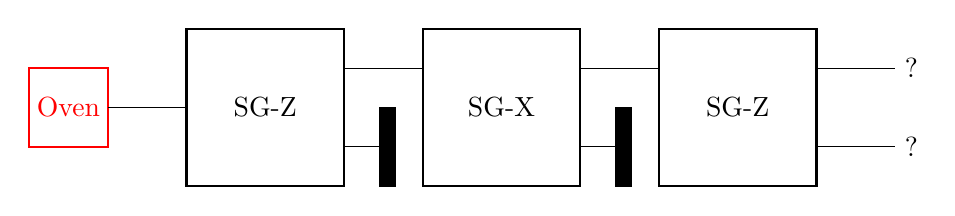
\begin{tikzpicture}
        \draw[red, thick] (0, 0) -- (1, 0) -- (1, 1) -- (0, 1) -- cycle;
        \node[red] at (0.5, 0.5) {Oven};
        \draw[] (1, 0.5) -- (2, 0.5);
        \draw[thick] (2, -0.5) -- (2, 1.5) -- (4, 1.5) -- (4, -0.5) -- cycle;
        \node[] at (3, 0.5) {SG-Z};
        \draw[] (4, 1) -- (5, 1);
        \draw[] (4, 0) -- (4.45, 0);
        \filldraw[fill = black, draw = black] (4.45, -0.5) -- (4.45, 0.5) -- (4.65, 0.5) -- (4.65, -0.5) -- cycle;
        \draw[thick] (5, -0.5) -- (5, 1.5) -- (7, 1.5) -- (7, -0.5) -- cycle;
        \node[] at (6, 0.5) {SG-X};
        \draw[] (7, 1) -- (8, 1);
        \draw[] (7, 0) -- (7.45, 0);
        \filldraw[fill = black, draw = black] (7.45, -0.5) -- (7.45, 0.5) -- (7.65, 0.5) -- (7.65, -0.5) -- cycle;
        \draw[thick] (8, -0.5) -- (8, 1.5) -- (10, 1.5) -- (10, -0.5) -- cycle;
        \node[] at (9, 0.5) {SG-Z};
        \draw[] (10, 1) -- (11, 1);
        \draw[] (10, 0) -- (11, 0);
        \node[right] at (11, 1) {?};
        \node[right] at (11, 0) {?};
    \end{tikzpicture}
   \caption{Cartoon of a sequential Stern-Gerlach experiment. First, the z-component of the spin of particles coming out of the oven area measured. The $S_z = +\frac{\hbar}{2}$ (spin up/$\ket{\uparrow}$) particles are allowed to go through, while the $S_z = -\frac{\hbar}{2}$ (spin down/$\ket{\downarrow}$) particles are blocked. Then, the $x$-component of the spin is measured, with the $S_x = +\frac{\hbar}{2}$ (spin right/$\ket{+}$) particles allowed to go through, and the $S_x = -\frac{\hbar}{2}$ (spin left/$\ket{-}$) particles blocked. Finally, the $z$-component of the spin is measured again.}
    \label{fig-SGsequential}
\end{figure}

Let us carry out the calculation to deduce what we would find at the output ports of the above experiment. In the first $S_z$ measurement, there is a 50/50 probability of measuring the spin to be spin-up, and so 50\% of the original particles go through. Then recalling that $\ket{\pm} = \frac{\ket{\uparrow} \pm \ket{\downarrow}}{\sqrt{2}}$, we have that $\ket{\uparrow} = \frac{\ket{+} + \ket{-}}{\sqrt{2}}$ and so we find in the second measurement that $p(+) = \abs{\braket{+}{\uparrow}}^2 = \frac{1}{2}$ And $p(-) = \abs{\braket{-}{\uparrow}}^2 = \frac{1}{2}$ (we may use the non-degenerate formulation of the Born rule here) so half of the particles go through - one quarter of the original particles from the oven. Now, we note something interesting; when we do the probability calculation for the third measurement, we find $p(\uparrow) = \abs{\braket{\uparrow}{+}}^2 = \frac{1}{2}$ and $p(\downarrow) = \abs{\braket{\downarrow}{+}}^2 = \frac{1}{2}$, so we find that one eigth of the original particles from the oven are present at each of the two output ports. Classically, this is quite strange - a classical measurement does not disturb the system, so when we measure the $z$-component of spin for the second time, we should expect to get 100\% spin-up (as we post-selected on spin-up in the first measurement)! But this is indeed not what happens quantum mechanically - in QM, measurements physically change the state of the system, so there are physical observables that are incompatible with each other (that is, there value cannot be simulataneously precisely known). Let us formalize this notion with a definition:

\begin{defbox}{: Compatible observables}
    Two observables $A, B$ are \emph{compatible} if:
    \begin{equation}
        [A, B] \coloneqq AB - BA = 0.
    \end{equation}
\end{defbox}

The $[\cdot, \cdot]$ appearing in the above definition is known as the \emph{commutator}, and can be interpreted as quantifying the extent to which two objects commute.

Compatible observables are characterized by the following properties:
\begin{itemize}
    \item The probability $p(a, b)$ for obtaining the outcome $a$ for $A$ and $b$ for $B$ is independent of the order of measurement.
    \item Compatible measurements do not disturb one another; suppose $A$ is measured with outcome $a$ and then $B$ with outcome $b$. If $A$ is measured a second time, then the outcome is $a$ again, with certainty.
\end{itemize}

These properties follow as the result of the following Lemma:

\begin{lembox}{}
    Compatible observables have a joint eigenbasis.
\end{lembox}

\begin{proof}
    Choose an (orthonormal) eigenbasis $\set{\ket{a}}$ of $A$. Since $[A, B] = 0$, it follows that $\bra{a'}[A, B]\ket{a} = 0$ and so:
    \begin{equation}
        0 = \bra{a'}[A, B]\ket{a} = (\bra{a'}A)B\ket{a} - \bra{a'}B(A\ket{a}) = (a' - a)\bra{a'}B\ket{a}
    \end{equation}
    So if $a \neq a'$, it follows that $\bra{a'}B\ket{a} = 0$. If $A$ is non-degenerate, we are immediately done as $B$ is diagonal in the basis $\set{\ket{a}}$ and hence it is also an eigenbasis of $B$. However, if $A$ is degenerate then $a = a'$ is possible for distinct $\ket{a}, \ket{a'}$. This means that $B$ is block diagonal in the basis $\set{\ket{a}}$. For example in the case where $A$ has two degenerate eigenvalues $a_1$ and three degenerate eigenvalues $a_2$, $B$ in this eigenbasis will be block diagonal with two blocks:
    \begin{equation}
        \vcenter{\hbox{\begin{tikzpicture}
            \node[] at (0, 0) {$A = \m{a_1 & 0 & & & \\ 0 & a_1 & & & \\ & & a_2 & 0 & 0 \\ & & 0 & a_2 & 0 \\ & & 0 & 0 & a_2}$};
            \node[font=\large] at (1.05, 0.7) {0};
            \node[font=\large] at (-0.6, -0.4) {0};
            \draw[dashed] (-1.1, 0.175) -- (-0.1, 0.175) -- (-0.1, 1.125) -- (-1.1, 1.125) -- cycle;
            \draw[dashed] (0.2, -1.1) -- (1.9, -1.1) -- (1.9, 0.175) -- (0.2, 0.175) -- cycle;

            \node[] at (5, 0) {$B = \m{\phantom{a_1} & \phantom{0} & & & \\ \phantom{0} & \phantom{a_1} & & & \\ & & \phantom{a_2} & \phantom{0} & \phantom{0} \\ & & \phantom{0} & \phantom{a_2} & \phantom{0} \\ & & \phantom{0} & \phantom{0} & \phantom{a_2}}$};
            \node[font=\large] at (1.05+5, 0.7) {0};
            \node[font=\large] at (-0.6+5, -0.4) {0};
            \draw[dashed, fill=black] (-1.1+5, 0.175) -- (-0.1+5, 0.175) -- (-0.1+5, 1.125) -- (-1.1+5, 1.125) -- cycle;
            \draw[dashed, fill=black] (0.2+5, -1.1) -- (1.9+5, -1.1) -- (1.9+5, 0.175) -- (0.2+5, 0.175) -- cycle;

        \end{tikzpicture}}}
    \end{equation}
    Now, we borrow a a known theorem from linear algebra (the Spectral theorem) that a Hermitian matrix can be diagonalized with a unitary matrix - hence, there exists some unitary transformation $U$ (which will have a block-diagonal matrix representation consisting of blocks $U_1, U_2$ in the same location as the blocks of $B$) which diagonalizes $B$:
    \begin{equation}
        \vcenter{\hbox{\begin{tikzpicture}
            \node[] at (0, 0) {$U = \m{\phantom{a_1} & \phantom{0} & & & \\ \phantom{0} & \phantom{a_1} & & & \\ & & \phantom{a_2} & \phantom{0} & \phantom{0} \\ & & \phantom{0} & \phantom{a_2} & \phantom{0} \\ & & \phantom{0} & \phantom{0} & \phantom{a_2}}$};
            \node[font=\large] at (1.05, 0.7) {0};
            \node[font=\large] at (-0.6, -0.4) {0};
            \draw[dashed] (-1.1, 0.175) -- (-0.1, 0.175) -- (-0.1, 1.125) -- (-1.1, 1.125) -- cycle;
            \draw[dashed] (0.2, -1.1) -- (1.9, -1.1) -- (1.9, 0.175) -- (0.2, 0.175) -- cycle;
            \node[] at (-0.6, 0.65) {$U_1$};
            \node[] at (1.05, -0.4625) {$U_2$};
        \end{tikzpicture}}}
    \end{equation}

    Then, we have that $UAU^\dag = A$ (consider that the blocks of $U$ act on the eigenspaces of $A$ independently, and then cancel to the identity by the condition $UU^\dag = I$, thus leaving $A$ invariant) and $UBU^\dag = B'$ is diagonal. In other words, the basis $\set{U^\dag \ket{a}}$ is a joint eigenbasis of $A, B$ and we are done.
\end{proof}

Since $A, B$ share an eigenbasis, in this same basis the projectors corresponding to the various are diagonal. It therefore follows that:
\begin{equation}
    [\Pi_{A, a}, \Pi_{B, b}] = [\Pi_{A, a}, B] = [A, \Pi_{B, b}] = 0.
\end{equation}

From this fact, we can argue the two properties of compatible observables. First, we show that the probability $p(a, b)$ for obtaining the outcome $a$ for $A$ and $b$ for $B$ is independent of the order of measurement.

Suppose we measure $A$ first, then $B$. Then the post measurement state after the first measurement is $\frac{\Pi_{a, a}\ket{\psi}}{\sqrt{\bra{\psi}\Pi_{A, a}\ket{\psi}}}$, by the Dirac postulate. The probability to measure $b$ in the second measurement (given that we measured $a$ in the first measurement) is then given by the Born rule to be:
\begin{equation}
    p(b\vert a) = \frac{\bra{\psi}\Pi_{A, a}\Pi_{B, b}\Pi_{A, a}\ket{\psi}}{\bra{\psi}\Pi_{A, a}\ket{\psi}}
\end{equation}
The probability for measuring $a$ and $b$ is then calculated as:
\begin{equation}
    \begin{split}
        p(a, b) = p(a \cap b) = p(b \vert a)p(a) &= \left(\frac{\bra{\psi}\Pi_{A, a}\Pi_{B, b}\Pi_{A, a}\ket{\psi}}{\bra{\psi}\Pi_{A, a}\ket{\psi}}\right)\bra{\psi}\Pi_{A, a}\ket{\psi}
        \\ &= \bra{\psi}\Pi_{A, a}\Pi_{B, b}\Pi_{A, a}\ket{\psi}
        \\ &= \bra{\psi}\Pi_{A, a}^2\Pi_{B, b}\ket{\psi}
        \\ &= \bra{\psi}\Pi_{A, a}\Pi_{B, b}\ket{\psi}
    \end{split}
\end{equation}
where in the second-to-last equality we use that the projectors commute, and in the last equality we use that projectors are idempotent. If we measure $B$ first and then $A$ and go through the same calculation (simply by interchanging $A \leftrightarrow B$), we find the exact same expression, and therefore we conclude that $p(a, b)$ is indepdendent of measurement order.

Let us also demonstrate that the compatible measurements do not disturb one another. If we measure $A$ with outcome $a$, we have $\ket{\psi} \mapsto \ket{a}$ with $A \ket{a} = a\ket{a}$. If we then measure $B$, we have $\ket{a} \mapsto \frac{\Pi_{B, b}\ket{a}}{\sqrt{\bra{a}\Pi_{B, b}\ket{a}}}$. Using the fact that $A, \Pi_{B, b}$ commute we then observe:
\begin{equation}
    A\left( \frac{\Pi_{B, b}\ket{a}}{\sqrt{\bra{a}\Pi_{B, b}\ket{a}}}\right) = \frac{\Pi_{B, b}A\ket{a}}{\sqrt{\bra{a}\Pi_{B, b}\ket{a}}} = a\left( \frac{\Pi_{B, b}\ket{a}}{\sqrt{\bra{a}\Pi_{B, b}\ket{a}}}\right)
\end{equation}
so the post-measurement state after measuring $B$ is still an eigenstate of $A$, with the same eigenvalue $a$!

We note an important example of compatible observables. For all observables $A$, it holds that $[A^n, A^m] = 0$ for all $n, m \in \NN$. In other words, all of $\set{A^k, k \in \NN}$ can be simultaneously measured. In the homework, you will be tasked with considering the relationship between the expectation values $\abs{A^k}_\psi = \bra{\psi}A^k\ket{\psi}$ of observables $A^k$, and the measurement probabilities $p(i) = \abs{\braket{b_i}{\psi}}^2$ where $\set{\ket{b_i}}_i$ is the eigenbasis of $A$. 

Alongside the discussion of compatible observables runs the consideration of incompatible observables:

\begin{defbox}{: Incompatible observables}
    Two observables $A, B$ are \emph{incompatible} if:
    \begin{equation}
        [A, B] \neq 0.
    \end{equation}
\end{defbox}
Incompatible observables have the properties that: 
\begin{itemize}
    \item The probability $p(a, b)$ for obtaining the outcome $a$ for $A$ and $b$ for $B$ is generally dependent of the order of measurement.
    \item Incompatible measurements disturb one another.
\end{itemize}
A good example is our motivating example of the $S_z$ and $S_x$ measurements at the beginning of this section. Indeed, $[S_z, S_x] = i\hbar S_y \neq 0$ and so the two observables are incompatible.  

\subsection{Position and Momentum}
In this section, we discuss two key examples of observables - namely position and momentum. We discuss their eigenstates, which take on a continuous range. We discuss their commutation relation which is the axiomatic foundation of how they relate. We derive the momentum operator in the position basis, and show that position and momentum wavefunctions relate via a Fourier transform. Finally, we will derive the famous Heisenberg uncertainty relation.

The spin observables we have considered so far in this course have taken on discrete values (e.g. the eigenvalues of $S_z$ for a spin-1/2 particle are $\pm \frac{\hbar}{2}$). However, the eigenvalues of position and momentum are continuous; for example, a (free) particle in one dimension can have $x \in (-\infty, \infty)$. To handle this, we will content ourselves to generalize the finite-dimensional formalism to the infinite-dimensional setting in the natural way, sweeping the functional analytic details under the rug.

So, we consider the (one-dimensional) position operator $X$, with a complete and orthonormal set of eigenstates $\set{\ket{x}}$ that satisfy $X\ket{x} = x\ket{x}$ with $x$ the position eigenvalue. The resolution of identity (as we discussed in a previous section) reads $\int dx \dyad{x}{x} = \mathbb{I}$, and the orthonormality relation reads $\braket{x'}{x} = \delta(x - x')$. 

We can also consider the (one-dimensional) linear momentum operator $P$, which has a complete and orthonormal set of eigenstates $\set{\ket{p}}$ that satisfy $P\ket{p} = p\ket{p}$ with $p$ the momentum eigenvalue. The resolution of identity reads $\int dp \dyad{p}{p} = \mathbb{I}$ and the orthonormality relation reads $\braket{p'}{p} = \delta(p - p')$. 

We define the position and momentum wavefunctions $\psi(x)/\tilde{\psi}(p)$ as the expansion coefficients of a state $\ket{\psi}$ in the position/momentum bases:
\begin{equation}\label{eq-positionwf}
    \ket{\psi} = \left(\int dx \dyad{x}{x}\right)\ket{\psi} = \int dx \braket{x}{\psi} \ket{x} = \int dx \psi(x) \ket{x}
\end{equation}
\begin{equation}\label{eq-momentumwf}
    \ket{\psi} = \left(\int dp \dyad{p}{p}\right) \ket{\psi} = \int dp \braket{p}{\psi} \ket{p} = \int dp \tilde{\psi}(p) \ket{p}.
\end{equation}

Having introduced some operators with continuous spectra, let us return briefly back to our example of higher moments, namely expectation values of $X^n$. Calculating the expectation of $X$, we have:
\begin{equation}
   \avg{X}_\psi =  \bra{\psi}X\ket{\psi} = \int dx dy \braket{\psi}{x} \bra{x}X\ket{y} \braket{y}{\psi} = \int dx dy \psi^*(x) y\delta(x - y) \psi(y) = \int dx x\abs{\psi(x)}^2
\end{equation}
which is the average position of the state $\ket{\psi}$. Calculating the expectation of $X^2$, we have:
\begin{equation}
    \avg{X^2}_\psi = \bra{\psi}X\ket{\psi} = \int x^2 \abs{\psi(x)}^2
\end{equation}
which gives information about the width - $\abs{\psi(x)}^2$ has the interpretation of a probability density in position space, and the expectation values of $X^n$ gives information about the distribution. For example the variance yields a measure of the deviation from the mean value:
\begin{equation}
    \avg{(\Delta X)^2}_\psi = \avg{(X - I\avg{X})^2}_\psi = \avg{X^2}_\psi - \avg{X}^2_\psi
\end{equation} 
We can also calculate the skewedness $\avg{(\Delta X)^3}$, which is a measure of how asymmetric the distribution is, and so on. All moments taken together contain the same information\footnote{Well, not quite, there are some \href{https://math.stackexchange.com/questions/1790858/two-random-variables-with-same-moments}{pathological counterexamples}} as the probability density $\abs{\psi(x)}^2$. 

Having now a better understanding of moments and continuous probability densities, let us discuss the fundamental relationship between position and momentum.

\begin{axiombox}{: Canonical commutation relations}
    The commutation relations between position and momentum are:
    \begin{equation}
        [X_i, X_j] = 0, \quad [P_i, P_j] = 0, \quad [X_i, P_j] = i\hbar\delta_{ij}\mathbb{I}
    \end{equation}
    where the subscript denotes the component of position/momentum, and $\delta_{ij}$ is the Kronecker delta.
\end{axiombox}
Note that there is a noteworthy relationship between classical and quantum mechanics:
\begin{equation}
    [\cdot, \cdot]_{\text{classical}} \mapsto \frac{[\cdot, \cdot]}{i\hbar}
\end{equation}
where $[\cdot, \cdot]_{\text{classical}}$ denotes the Poisson bracket.

We can understand the notion of momentum as a generator of translations using these commutation relations. To this end, let us define:

\begin{defbox}{: Translation operator}
    The translation operator is defined as the following imaginary exponential:
    \begin{equation}
        \mathcal{T}(\Delta x) \coloneqq e^{-i\frac{P}{\hbar}\Delta x}
    \end{equation}
    where $P$ is the momentum operator and $\Delta x$ some real number.
\end{defbox}

We now claim that the translation operator lives up to its namesake:

\begin{propbox}{}
    The translation operator translates a position eigenket, that is:
    \begin{equation}
        \mathcal{T}(\Delta x)\ket{x} = \ket{x + \Delta x}
    \end{equation}
\end{propbox}

\begin{proof}
    Let us Taylor expand the translation operator (recalling the Taylor expansion of the exponential - of course, this is how exponentials of operators are formally defined):
    \begin{equation}
        \mathcal{T}(\Delta x) = \II - i\frac{P}{\hbar}\Delta x + O((\Delta x)^2).
    \end{equation}
    Furthermore, let us recall the eigenvalue equation $X\ket{x} = x\ket{x}$. Now, we consider $\mathcal{T}(\Delta x)\ket{x}$:
    \begin{equation}
        \begin{split}
            X\mathcal{T}(\Delta x)\ket{x} &= X\left(\II - i\frac{P}{\hbar}\Delta x + O((\Delta x)^2)\right)\ket{x}
            \\ &= X\ket{x} - i\frac{\Delta x}{\hbar}XP\ket{x} + O((\Delta x)^2)
            \\ &= x\ket{x} - i\frac{\Delta x}{\hbar}\left(i\hbar \mathbb{I} + PX\right)\ket{x} + O((\Delta x)^2)
            \\ &= x\ket{x} + \Delta x\ket{x} - i\frac{\Delta x}{\hbar}P x\ket{x} + O((\Delta x)^2)
            \\ &= (x + \Delta x)\left(\mathbb{I} - i\frac{P}{\hbar}\Delta x\right)\ket{x} + O((\Delta x)^2)
            \\ &=  (x + \Delta x)\mathcal{T}(\Delta x)\ket{x} + O((\Delta x)^2)
        \end{split}
    \end{equation}
    where in the third equality we note the application of the canonical commutation relation. Also note in the fifth equality we introduce a term $\propto (\Delta x)^2$ but we may do this freely as such terms are absorbed by $O((\Delta x)^2)$. The conclusion is (up to terms of order $(\Delta x)^2$) that $\mathcal{T}(\Delta x)\ket{x}$ is an eigenket of position with eigenvalue $x + \Delta x$  and so $\mathcal{T}(\Delta x)\ket{x} = \ket{x + \Delta x}$. So, for infinitesimal translations (for which we can neglect terms $O((\Delta x)^2)$) the claim holds. We are then able to conclude the result for general translations by considering a general translation as a composition of many infinitesimal ones.
\end{proof}

Note: We could instead have posited as an axiom the above property of the translation operator/momentum as a generator of translations, and from there derived the canonical commutation relations (and in fact Sakurai derives things in this order) - there is not a huge difference as one set of relations can always be derived from the other.

Using the translation operator, we can derive the form of the momentum operator in the position basis - this will be useful for deriving the form of the Schrodinger equation in the position basis from the general basis-independent equation, as we will do in the next part of the course.

\begin{propbox}{: Momentum operator in position basis}
    For a general state $\ket{\alpha}$, we have:
    \begin{equation}
        \bra{x}P\ket{\alpha} = -i\hbar\dpd{}{x}\braket{x}{\alpha}
    \end{equation}
\end{propbox}

\begin{proof}
We consider operating the translation operator $\mathcal{T}(\Delta x)$ on the general state $\ket{\alpha}$. We consider small $\Delta x$ so as to neglect terms of order $(\Delta x)^2$ and higher:
\begin{equation}
    \begin{split}
        \left(\mathbb{I} - i\frac{P}{\hbar}\Delta x\right)\ket{\alpha} &= \mathcal{T}(\Delta x)\ket{\alpha} 
        \\ &= \int dx' \mathcal{T}(\Delta x)\ket{x'}\braket{x'}{\alpha}
        \\ &= \int dx' \ket{x' + \Delta x} \braket{x'}{\alpha}
        \\ &= \int dx' \ket{x'}\braket{x' - \Delta x}{\alpha} 
        \\ &= \int dx' \ket{x'}\left(\braket{x'}{\alpha} - \Delta x'\dpd{}{x'}\braket{x'}{\alpha}\right)
    \end{split}
\end{equation}
where in the second equality we have inserted the resolution of the identity, in the third equality we use the translation property derived above, in the fourth equality we make the substitution $x' \to x' - \Delta x$, and in the fifth equality we Taylor expand $\braket{x' - \Delta x}{\alpha}$. Now, if we equate order $\Delta x$ terms on both sides, we obtain:
\begin{equation}
    -i\frac{P}{\hbar}\Delta x\ket{\alpha} = \int dx' \ket{x'}(-\Delta x'\dpd{}{x'}\braket{x'}{\alpha})
\end{equation}
Multiplying both sides by $i\hbar\bra{x}$ and cancelling out the $\Delta x$s:
\begin{equation}
    \bra{x}P\ket{\alpha} = \int dx' \braket{x}{x'}\left(-i\hbar \dpd{}{x'}\braket{x'}{\alpha}\right) = \int dx' \delta(x - x')\left(-i\hbar \dpd{}{x'}\braket{x'}{\alpha}\right)
\end{equation}
the delta function picks out $x' = x$ in the integral and so we obtain:
\begin{equation}
    \bra{x}P\ket{\alpha} = -i\hbar\dpd{}{x}\braket{x}{\alpha}
\end{equation}
as claimed.
\end{proof}

With this representation of the momentum operator derived, we are now able to show that the position and momentum space wavefunctions (Eqs. \eqref{eq-positionwf}, \eqref{eq-momentumwf}) are related via a Fourier transform.

\begin{propbox}{: Fourier transform between position and momentum}
    Given a state $\ket{\psi}$, its momentum wavefunction $\tilde{\psi}(p)$ and position wavefunction $\psi(x)$ are related by a Fourier transform, that is:
    \begin{equation}
        \tilde{\psi}(p) \propto \int dx e^{-ipx/\hbar}\psi(x).
    \end{equation}
\end{propbox}

\begin{proof}
    Recall that:
    \begin{equation}
        \tilde{\psi}(p) = \braket{p}{\psi} = \int dx \braket{p}{x}\braket{x}{\psi} = \int dx \braket{p}{x} \psi(x).
    \end{equation}
    by definition of the momentum/position wavefunctions and using the resolution of the identity. So, it suffices to show that $\braket{p}{x} \propto e^{-ipx/\hbar}$.
    
    We recall the representation $\bra{x}P\ket{\alpha} = -i\hbar\dpd{}{x}\braket{x}{\alpha}$ that we derived just before. Now, set $\ket{\alpha} = \ket{p}$ a momentum eigenstate. We then have that:
    \begin{equation}
        \bra{x}P\ket{p} = \bra{x}p\ket{p} = p\braket{x}{p}
    \end{equation}
    using the eigenvalue equation, and also that:
    \begin{equation}
        \bra{x}P\ket{p} = -i\hbar\dpd{}{x}\braket{x}{p}
    \end{equation}
    using our previous result. We therefore obtain the equation:
    \begin{equation}
        p\braket{x}{p} = -i\hbar\dpd{}{x}\braket{x}{p}
    \end{equation}
    which is a first-order ODE which is easily solved:
    \begin{equation}
        \braket{x}{p} \propto e^{ipx/\hbar}
    \end{equation}
    and therefore:
    \begin{equation}
        \braket{p}{x} = \braket{x}{p}^* \propto e^{-ipx/\hbar}
    \end{equation}
    and so we are done.
\end{proof}

There is one detail we skipped in the above proof; namely, the normalization of $\braket{x}{p}$. If we want to determine $N$ in $\braket{x}{p} = Ne^{ipx/\hbar}$, we can consider:
\begin{equation}
    \begin{split}
        \delta(x - x') = \braket{x}{x'} &= \int dp \braket{x}{p}\braket{p}{x'}
        \\ &= \abs{N}^2\int dp e^{ip(x - x')/\hbar}
        \\ &= \abs{N}^2 2\pi\hbar \delta(x - x')
    \end{split}
\end{equation}
where the last integral is a standard one in Fourier Analysis. comparing the two sides of the equation, we can conclude:
\begin{equation}
    N = \frac{1}{\sqrt{2\pi\hbar}}.
\end{equation}

Now, we move to a discussion of uncertainty relations - the most famous of which is the Heisenberg uncertainty relation of position and momentum. This relation has key physical implications - for example being responsible for the size scale of atoms. Let us explore the HUP with an example before going into its formal derivation.

We consider a variation on the sequential Stern-Gerlach experiment involving position and momentum; in other words, a single-slit diffraction experiment\footnote{This may be familiar to you from a homework assignment in PHYS 200 - if not, we go through it again briefly here together.}!

\begin{figure}[htbp]
    \centering
    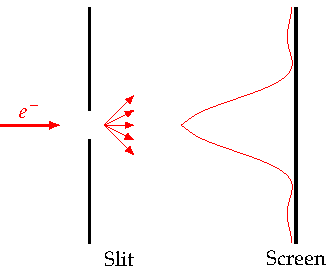
\includegraphics[]{Images/fig-singleslitdiffraction.pdf}
    
    \caption{Cartoon of a single-slit diffraction experiment. A beam of electrons is fired through a slit, which amounts to a position measurement of the electrons at the slit. The electrons then propogate until they hit the screen, which results in a diffraction pattern (after many electrons are fired) - the momentum of the electron at the slit can then be inferred from the position which the electron hits the screen.}
    \label{fig-singleslitdiffraction}
\end{figure}

To understand this experiment quantum-mechanically, we consider that the position of electrons is measured as they pass through a slit; at this point, a reasonable description of the position wavefunction of the electrons is the uniform wavefunction extending across the slit (which we assume to have width $2d$):
\begin{equation}
    \psi(x) = \begin{cases}
        \frac{1}{\sqrt{2d}} & -d \leq x \leq d
        \\ 0 & \text{otherwise}
    \end{cases}
\end{equation}

We can then take the Fourier transform to find the momentum wavefunction:
\begin{equation}
    \tilde{\psi}(p) = \frac{1}{\sqrt{2\pi\hbar}}\int_{-\infty}^\infty dx \psi(x)e^{-ipx/\hbar} = \sqrt{\frac{\hbar}{\pi d}}\frac{\sin(\frac{pd}{\hbar})}{p}
\end{equation}
(we skip the algebra here; but this is one special case where one can easily take the Fourier transform. Try it!) The modulus square of this momentum wavefunction yields the diffraction pattern that we see on the experiment screen.

This experiment is interesting to us here because it shows us how both position and momentum cannot be precisely known; Looking at the expression for $\tilde{\psi}(p)$ above, we see that if we decrease the slit size $d$ (i.e. we are more certain of the position of the electron) then the momentum wavefunction spreads out and we are less certain of it (and vise versa) - see Fig. \ref{fig-FTHUP} for a graphical sketch of this.

\begin{figure}[htbp]
    \centering
    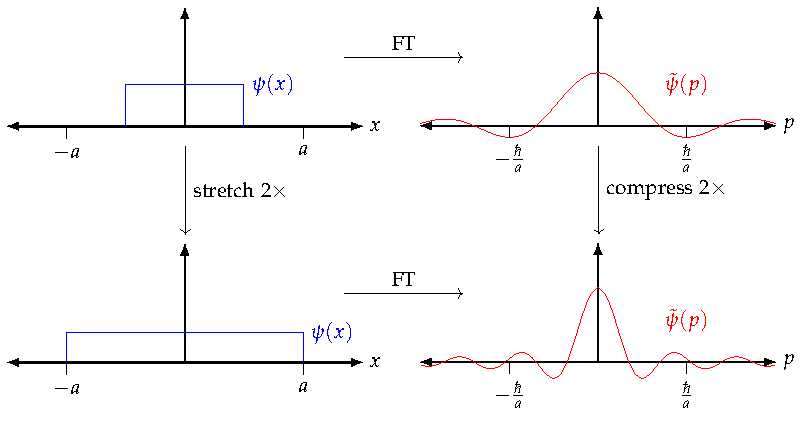
\includegraphics[]{Images/fig-FTHUP.pdf}
    \caption{Graphical Depiction of the impact of varying the width of the position wavefunction (slit size) on the momentum wavefunction (diffraction pattern width). As we stretch out the position wavefunction (and the position of the electron becomes more uncertain), the momentum wavefunction compresses, and we are more certain about the momentum of the electron at the slit. However, the position and momentum uncertainty cannot be decreased simultaneously - something that is rigorously characterized in the Heisenberg Uncertainty Relation.}
    \label{fig-FTHUP}
\end{figure}

Let us now derive the HUP. To begin, we will prove a more general uncertainty principle between operators. To this end, we will require a Lemma concerning inner products of vectors:

\begin{lembox}{: Cauchy-Shwartz inequality}
    Let $\ket{\alpha}, \ket{\beta}$ be two vectors. Then,
    \begin{equation}
        \braket{\alpha}{\alpha}\braket{\beta}{\beta} \geq \abs{\braket{\alpha}{\beta}}^2.
    \end{equation}
\end{lembox}
\begin{proof}
    Since $\braket{v}{v} \geq 0$ for any vector $\ket{v}$, it follows that:
    \begin{equation}
        (\bra{\alpha} + \lambda^*\bra{\beta})(\ket{\alpha} + \lambda\ket{\beta}) \geq 0
    \end{equation}
    for all $\lambda \in \CC$. Now, set $\lambda = -\frac{\braket{\beta}{\alpha}}{\braket{\beta}{\beta}}$. Multiplying out the resulting expression, we obtain:
    \begin{equation}
        \braket{\alpha}{\alpha}\braket{\beta}{\beta} - \abs{\braket{\alpha}{\beta}}^2 \geq 0
    \end{equation}
    which proves the claim.
\end{proof}

With this Lemma under our belt, we have the tools in place to prove the following:

\begin{thmbox}{: General uncertainty relation}
    Let $A, B$ be two observables, and define $\Delta A \coloneqq A - \avg{A}_\psi I$, $\Delta B \coloneqq B - \avg{B}_\psi I$, (where the expectation value is taken with respect some state $\ket{\psi}$). It then follows that:
    \begin{equation}
        \avg{(\Delta A)^2}_\psi\avg{(\Delta B)^2}_\psi \geq \frac{1}{4}\abs{\avg{[A, B]}_\psi}^2.
    \end{equation}
\end{thmbox}
\begin{proof}
    Let $\ket{\alpha} = (\Delta A)\ket{\psi}$ and $\ket{\beta} = (\Delta B)\ket{\psi}$. Applying Cauchy-Shwartz, we obtain:
    \begin{equation}\label{eq-CSapplied}
        \avg{(\Delta A)^2}_\psi\avg{(\Delta B)^2}_\psi \geq \abs{\avg{\Delta A\Delta B}_\psi}^2.
    \end{equation}
    Now, notice that we can decompose:
    \begin{equation}
        \Delta A \Delta B = \frac{1}{2}[\Delta A, \Delta B] + \frac{1}{2}\{\Delta A, \Delta B \}
    \end{equation}
    Where $\{\Delta A, \Delta B\} = \Delta A\Delta B + \Delta B\Delta A$ denotes the \emph{anti-commutator} of $\Delta A$ and $\Delta B$. Now, we claim that $\bra{\psi}[\Delta A, \Delta B]\ket{\psi}$ is imaginary. To see this, note:
    \begin{equation}
        [\Delta A, \Delta B]^\dag = (\Delta A \Delta B - \Delta B \Delta A)^\dag = \Delta B \Delta A - \Delta A \Delta B = -[\Delta A, \Delta B]
    \end{equation}
    where we have used that $\Delta A, \Delta B$ are Hermitian, and that $(AB)^\dag = B^\dag A^\dag$ (this can be proven easily from the definition of the adjoint using the dual correspondence - it is a good exercise to check it)! From the above equation, we obtain:
    \begin{equation}
        (\bra{\psi}[\Delta A, \Delta B]\ket{\psi})^* = -\bra{\psi}[\Delta A, \Delta B]\ket{\psi}
    \end{equation}
    from which we would conclude that $\bra{\psi}[\Delta A, \Delta B]\ket{\psi}$ must be purely imaginary. 

    We can also verify that $\bra{\psi}\{\Delta A, \Delta B\}\ket{\psi}$ is real (check)! The upshot is then that we can write:
    \begin{equation}
        \avg{\Delta A\Delta B}_\psi = \frac{1}{2}\avg{[\Delta A, \Delta B]}_\psi + \frac{1}{2}\avg{\{\Delta A, \Delta B\}}_\psi
    \end{equation}
    with the first term purely imaginary, and the second term purely real. Then, using that for a complex number $z = a + bi$ that the modulus square is $\abs{z}^2 = \abs{a}^2 + \abs{b}^2$, we find:
    \begin{equation}
        \abs{\avg{\Delta A\Delta B}_\psi}^2 = \frac{1}{4}\abs{\avg{[\Delta A, \Delta B]}_\psi}^2 + \frac{1}{4}\abs{\avg{\{\Delta A, \Delta B\}}_\psi}^2 \geq \frac{1}{4}\abs{\avg{[\Delta A, \Delta B]}_\psi}^2
    \end{equation}
    where the last inequality follows from both terms being positive. Combining this result with \eqref{eq-CSapplied}, we find:
    \begin{equation}
        \avg{(\Delta A)^2}_\psi\avg{(\Delta B)^2}_\psi \geq \frac{1}{4}\abs{\avg{[\Delta A, \Delta B]}_\psi}^2
    \end{equation}
    which is exactly what we wished to show.
\end{proof}

\begin{corbox}{: Heisenberg uncertainty principle}
    The position operator $X$ and momentum operator $P$ (in the same direction) satisfy:
    \begin{equation}
        \avg{(\Delta X)^2}_\psi\avg{(\Delta P)^2}_\psi \geq \frac{\hbar^2}{4}
    \end{equation}
\end{corbox}
\begin{proof}
    This follows immediately by setting $A = X, B = P$ in the general uncertainty relation, and applying the canonical commutation relation $[X, P] = i\hbar \mathbb{I}$. 
\end{proof}

Having now proven the Heisenberg uncertainty relation, it may be of interest to ask which wavefunctions saturate it; that is, for which $\ket{\psi}$ does it follow that:
\begin{equation}
    \avg{(\Delta X)^2}_\psi\avg{(\Delta P)^2}_\psi = \frac{\hbar^2}{4}?
\end{equation} 

\begin{propbox}{: Gaussian wavepackets saturate the HUP}
    Gaussian Wavepackets, that is, states with position wavefunctions:
    \begin{equation}
        \braket{x}{\psi} = (2\pi d^2)^{-1/4}e^{-\frac{x^2}{4d^2}}
    \end{equation}
    saturate the Heisenberg uncertainty principle.
\end{propbox}

\begin{figure}[htbp]
    \centering
    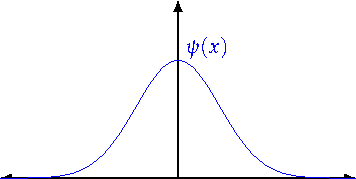
\includegraphics[]{Images/fig-Gaussian.pdf}
    \caption{Plot of a Gaussian wavefunction (with mean zero).}
    \label{fig-Gaussian}
\end{figure}
\begin{proof}
    First, note that:
    \begin{equation}
        \avg{(\Delta A)^2} = \avg{(A - \avg{A}\mathbb{I})^2} = \avg{A^2 - 2\avg{A}A + \avg{A}^2\mathbb{I}} = \avg{A^2} - 2\avg{A}^2 + \avg{A}^2 = \avg{A^2} - \avg{A}^2
    \end{equation}
    So we calculate $\avg{A}_\psi$ and $\avg{A^2}_\psi$ for $A = X, P$. First, note that $\avg{X}_\psi = 0$ as the wavefunction is symmetric about $x = 0$ ($\psi(x) = \psi(-x)$). Therefore:
    \begin{equation}
        \avg{(\Delta X)^2}_\psi = \avg{X^2}_\psi = \int_{-\infty}^\infty dx x^2(2\pi d^2)^{-1/4}e^{-\frac{x^2}{4d^2}} = d^2
    \end{equation}
    Since $\dod{\psi(x)}{x}$ is anti-symmetric, $\avg{P}_\psi = 0$ and hence:
    \begin{equation}
        \avg{(\Delta P)^2}_\psi = \avg{P^2}_\psi = \int_{-\infty}^\infty dx\left((2\pi d^2)^{-1/4}e^{-\frac{x^2}{4d^2}}\right)\left(-i\hbar\dod{}{x}\right)^2\left((2\pi d^2)^{-1/4}e^{-\frac{x^2}{4d^2}}\right) = \frac{\hbar^2}{4d^2}
    \end{equation}
    where we have used the representation of the momentum operator in the position basis. We therefore conclude for Gaussian wavepackets that:
    \begin{equation}
        \avg{(\Delta X)^2}_\psi \avg{(\Delta P)^2}_\psi = \frac{\hbar^2}{4}
    \end{equation}
    and hence the claim is proven.
\end{proof}

Note that the above argument generalizes easily to the case where $\avg{X}_\psi \neq 0$ for the Gaussian wavepacket (i.e. a Gaussian shifted from the origin).
Actually, the relationship between Gaussian wavepackets and HUP saturation is even stronger.

\begin{propbox}{: HUP Saturation $\iff$ Gaussian Wavpackets}
    Gaussian wavepackets are the only wavefunctions which saturate the Heisenberg uncertainty principle.
\end{propbox}
\begin{proof}
    We have already shown Gaussian wavepackets $\implies$ HUP saturation in the previous proof. So, what is left to do is show that if the HUP is saturated, then the state must be a Gaussian wavepacket.

    First, we go back to our derivation of the general uncertainty principle, where we invoked the Cauchy-Shwartz inequality. It can be shown that the CS-inequality is saturated with equality if and only if $\ket{\alpha} = c\ket{\beta}$ for some $c \in \CC$ (i.e. the two vectors in question are linearly independent). Therefore, in the context of position and momentum, we require:
    \begin{equation}\label{eq-XPlineardep}
        (\Delta X)\ket{\psi} = c(\Delta P)\ket{\psi}
    \end{equation}
    for some complex $c$. Further, in our derivation we threw away the anti-commutator term; for minimum uncertainty we require that this term be zero, i.e. $\abs{\avg{\set{\Delta X, \Delta P}}}^2 = 0$. But we established in the uncertainty relation argument that this was real, so if it is zero, it follows that $c$ appearing in Eq. \eqref{eq-XPlineardep} is purely imaginary. Thereofre if we consider the ODE defined by Eq. \eqref{eq-XPlineardep} in the position basis, we obtain:
    \begin{equation}
        x\psi(x) = ci\hbar\dpd{}{x}\psi(x)
    \end{equation}
    where we have assumed $\avg{X}_\psi = \avg{P}_\psi = 0$ for simplicity (however this assumption can be relaxed - $\avg{X}$ will only shift the Gaussian some amount from the origin, and $\avg{P}$ will only tack on a physically irrelevant phase factor - check this if you like!). It can then be easily checked that (for imaginary $c$) that the solutions to the above ODE are Gaussians, which completes the proof of the claim.
\end{proof}

